\documentclass[12pt]{article}

%------------------------------------------------
% Page Layout
%------------------------------------------------
\usepackage[margin=1in]{geometry}
\setlength{\parskip}{0.6em}
\setlength{\parindent}{0pt}

%------------------------------------------------
% Fonts and Encoding
%------------------------------------------------
\usepackage[T1]{fontenc}
\usepackage[utf8]{inputenc}
\usepackage{lmodern}
\usepackage{comment}
\usepackage[table]{xcolor}

%------------------------------------------------
% Math Packages
%------------------------------------------------
\usepackage{amsmath,amssymb,amsfonts}
\usepackage{bm}

%------------------------------------------------
% Graphics and Figures
%------------------------------------------------
\usepackage{graphicx}
\usepackage{float}
\usepackage{subcaption}
\usepackage[compat=1.1.0]{tikz-feynman}

%------------------------------------------------
% Tables
%------------------------------------------------
\usepackage{booktabs}
\usepackage{tabularx}
\usepackage{pdflscape}

%------------------------------------------------
% Hyperlinks
%------------------------------------------------
\usepackage{hyperref}
\hypersetup{
    colorlinks=true,
    linkcolor=blue,
    citecolor=blue,
    urlcolor=blue
}

%------------------------------------------------
% Bibliography
%------------------------------------------------
\usepackage[numbers,sort&compress]{natbib}

%------------------------------------------------
% Section Formatting
%------------------------------------------------
\usepackage{titlesec}
\titleformat{\section}{\large\bfseries}{\thesection}{1em}{}
\titleformat{\subsection}{\normalsize\bfseries}{\thesubsection}{1em}{}
\usepackage{titling}


%------------------------------------------------
% Custom Commands
%------------------------------------------------

% Processes
\newcommand{\dd}{\mathrm{d}}
\newcommand{\ee}{\mathrm{e}}
\newcommand{\ii}{\mathrm{i}}
\newcommand{\muEtoEE}{\mu^- e^- \to e^- e^-}
\newcommand{\muToe}{\mu^- N \to e^- N}

% Common physics quantities
\newcommand{\CLFV}{\mathrm{CLFV}}
\newcommand{\BSM}{\mathrm{BSM}}
\newcommand{\SM}{\mathrm{SM}}
\newcommand{\GEANT}{\mathrm{GEANT4}}
\newcommand{\MuTwoE}{\mathrm{Mu2e}}

% Uncertainties
\newcommand{\dx}{\delta x}
\newcommand{\dy}{\delta y}
\newcommand{\dz}{\delta z}
\newcommand{\dpp}{\delta p}

%------------------------------------------------
% Setting paragraph indentation length
%------------------------------------------------
\setlength{\parindent}{15pt}

%------------------------------------------------
% Title Information
%------------------------------------------------

\title{A Proposal for a Sensitivity Study of
$\mu^- e^- \rightarrow e^-e^-$ in the Mu2e Experiment}

\author{
Andrew D. Boldy \\
\small Department of Physics and Astronomy, University of South Carolina
}

\date{\today}

%------------------------------------------------
\begin{document}
\setlength{\droptitle}{-2cm}
\maketitle
\setlength{\droptitle}{0pt}
%================================================
% Abstract
%================================================
\begin{abstract}

The Mu2e Experiment at Fermilab National Accelerator Laboratory provides a substantial opportunity to search for charged lepton flavor violating (CLFV) processes and thus probe physics beyond the Standard Model (BSM) in various conversion processes for the muon. The primary goal of Mu2e is to search for the coherent conversion of a negative muon into an electron in the field of a nucleus, $\muToe$, but the experimental environment may also provide sensitivity to additional processes involving bound muons, further increasing its importance to constraining BSM physics models in the CLFV regime.

This proposal for dissertation research introduces a full sensitivity study of the $\muEtoEE$ process in the Mu2e experimental design. The study will determine the extent to which the Mu2e detector, reconstruction system, and analysis framework can identify and characterize this process in the required experimental configuration. Achieving this primary goal mandates the development and validation of a dedicated event generator to be implemented into the simulation workflow an of event-selection criteria. The simulation products (including reconstruction of events) must be characterized and analyzed using both existing and in-development tools as will be analyzed upon actual running. These events must then be simulated alongside specific backgrounds including decay in orbit, cosmic rays, and other viable processes that may obscure the data and discrimination power of the analysis framework must be tested and statistically verified. A particular focus of the present work is the development of a geometric vertexing algorithm for reconstructing the common origin of the two electron tracks. 

Preliminary studies have incorporated a toy generator and required supporting code within the Mu2e computing environment, validated the generation of representative signal configurations in Monte Carlo truth and reconstruction products, and demonstrated the implementation of a rudimentary vertexing procedure to gain a preliminary estimate of the location for the common signal vertex. Future work will refine the current generator to more precisely implement the theoretical predictions for the process and implement a helical parameterization and full reconstruction data to improve resolution of the prediction for the vertex location. Then a mix of the process simulation with anticipated background to determine discrimination power will be introduced utilizing reconstruction uncertainties, statistical requirements, and computational considerations to validate the study.

The completed study will provide an estimate of the achievable Mu2e sensitivity to $\muEtoEE$ and predict optimal experimental condition requirements necessary to perform a statistically significant search for this process.

\end{abstract}

\tableofcontents
\clearpage

%================================================
% 1. Theoretical Motivation
%================================================

\section{Theoretical Motivation}\label{sec:Theory}

The Standard Model is the most thoroughly tested description of the fundamental components and interactions at the subatomic scale, describing almost all known phenomena at the smallest levels known. While not including gravitation, the Standard Model gives a fairly comprehensive description of the strong, weak, and electromagnetic forces their mediators, the vector bosons, and the matter particles as a $\text{SU(3)}_c \times \text{SU(2)}_L \times \text{U(1)}_Y$ gauge theory. 

While the Standard Model has been well tested, there is still a large array of theory and experimental work being done to test the limits and constraints of models that go beyond the Standard Model (BSM physics). One way to push the limits and determine the power of some of these BSM models is to extend the Standard Model via effective field theories. 

While there are many different types of effective field theories that can be used to produce models, one of particular interest that has been written about in several relevant paper and reviews (for instance, \cite{Brivio_2019} the 2019  review by Brivio and Trott, section 5.2) is Standard Model Effective Field Theory (SMEFT). In SMEFT, if the Standard Model typical form is defined as being a set of renormalizable operators of mass dimension four, $\mathcal{L}_\text{SM}^{(4)}$, we can write additional terms of higher dimensions that exist for higher energy systems that are not renormalizable in the typical sense. 
\begin{equation}\label{eqn:gen_SMEFT_Lagrangian}
\mathcal{L}_\text{SMEFT}=\mathcal{L}_{\text{SM}}^{(4)}+\mathcal{L}^{(5)}+\mathcal{L}^{(6)}+\mathcal{L}^{(7)}+\cdots
\end{equation}
where the raised index represents the mass dimension of those respective terms. To preserve the dimensionality of these higher dimensional terms in equation \ref{eqn:gen_SMEFT_Lagrangian}, the higher dimensional terms can be written as a linear combination of operators of dimension higher than four with a reciprocal energy scale ($\Lambda$) of increasing order. A general effective field theory extension of the Standard Model can then be written as
\begin{equation}\label{eqn:SMEFT_Lagrangian_expanded}
\mathcal{L}_{\text{SMEFT}} = \mathcal{L}^{(4)}_\text{SM}+\frac{1}{\Lambda}\sum_a C_a^{(5)}\mathcal{O}^{(5)}_a + \frac{1}{\Lambda^2}\sum_b C^{(6)}_b\mathcal{O}^{(6)}_b +\cdots= \mathcal{L}_{\text{SM}}+\sum_{D\geq 4}\frac{1}{\Lambda^{D-4}}\left[\sum_i C^{(D)}_i\mathcal{O}^{D)}_i\right]
\end{equation}

Here the $C_i$'s are called Wilson coefficients and are the fundamental components to be constrained by experimental data are vital in determining the reliability of effective descriptions of phenomena. The structure of the operators denoted by $\mathcal{O}^{(D)}_i$'s are dictated by the symmetries, most notably the gauge symmetry that defines the Standard Model interactions and Lorentz invariance. The energy scale determines when and how we might see possible terms arise in experimental results. It is in these extensions to the Standard Model at different energy scales that sometimes violations of previously believed invariance in the pure Standard Model processes may arise, as will be described specifically for charged lepton flavor.

\subsection{Flavor and Charged Lepton Flavor Violation}\label{subsec:FlavorCLFV}

In the Standard Model, the fundamental forces act on an array of matter particles, fermions of two types, quarks and leptons, and their antiparticles. These fermions, spin-1/2 particles with nonzero mass, can be described by their charge and by their generation in the Standard Model, but also, can be given another quantum number called "flavor." 

The quarks that comprise hadrons can be described according to the six flavors: up, charm, and top (the positively charged versions) and the down, strange, and bottom (the negatively charged ones). Since these charged particles are only found inside hadrons, that is, all observable combinations must be color-neutral by confinement in the strong interaction, explicit flavor content is determined based on mass of composite structures (particles or resonances). On the other side, there are the leptons, which like the quarks have six different types. These types can be described as three distinct "families," or similarly "lepton flavors." These families are electron-type, muon-type, and tau-type and consist of the so-named charged leptons as well as their uncharged neutrino counterparts.  

While many processes as described in the Standard Model have appeared to retain a conservation of this "flavor number," there is no explicit requirement that this is so from the gauge group of the Standard Model. Lepton flavor conservation arises as a byproduct, or "accidental symmetry," of the Standard Model \cite{CalibbiSignorelli2018CLFVIntro} arising from the particle content and lack of right handed neutrinos. Further, there has been evidence of lepton flavor violation in the neutrino sector on account of neutrino oscillations, the likelihood of such a transition being represented by the Pontecorvo-Maki-Nakagawa-Sakata (PMNS) matrix as predicted by Pontecorvo in 1968 \cite{Pontecorvo1968NeutrinoLeptonCharge}. The resulting calculable branching ratios for neutral flavor changing current is negligible on account of the Glashow-Iliopolous-Maiani (GIM) mechanism, on the order of $10^{-54}$ \cite{GIMMechanism1970} when calculated inside the Standard Model. However, this assumes that the Standard Model is complete, without additional terms from BSM physics models. As such, additional terms in an effective Lagrangian that may lift this symmetry restriction are of high interest, especially in experiments of the intensity regime.

In SMEFT, the dimension five operator, the Weinberg operator, \cite{Brivio_2019} violates lepton flavor number in the neutrino sector and after electroweak symmetry breaking, gives rise to the Majorana neutrino masses giving rise to neutrino mixing. However, this term does not produce any processes that result in charged lepton flavor violation. The next dimension up however, can produce such processes. The dimension six operators are the lowest order corrections that can produce CLFV processes.

Given that the electron has not been observed to decay as it is the lightest lepton, the decays of the charge muon ($\mu$) and tau ($\tau$) leptons are what experimentalists and theorists alike are primarily looking at. Given the longer lifetimes of the muon, these decays are can be viewed as more manageable for study. The lepton flavor conserving process of the Standard Model decay of the muon emits three particles according to the process 
\begin{equation}\label{SMMuonDecay}
    \mu^-\to e^-+\bar{\nu}_e+\nu_\mu
\end{equation}
with the Feynman diagram seen in figure \ref{feyn:SMMuonDecayFeynDiagram}

\begin{figure}[h!]
\begin{center}
\begin{tikzpicture} 
\begin{feynman}

    \vertex (mu) at (-2,0) {\(\mu^-\)};
    \coordinate (v1) at (0,0) {};

    \vertex (numu) at (2,1.5) {\(\nu_\mu\)};
    \coordinate (v2) at (2,-1.5) {};

    \vertex (e) at (4,-0.5) {\(e^-\)};
    \vertex (anue) at (4,-2.5) {\(\bar{\nu}_e\)};

    \diagram* {
        (mu) -- [fermion] (v1)
             -- [fermion] (numu),

        (v1) -- [boson, edge label=\(W^-\)] (v2),

        (v2) -- [fermion] (e),
        (v2) -- [anti fermion] (anue),
    };

\end{feynman}
\end{tikzpicture}
\caption{A Feynman diagram demonstrating the Standard Model decay of the muon. Note the final state being comprised of three particles and the conservation of lepton flavor.}
\label{feyn:SMMuonDecayFeynDiagram}
\end{center}
\end{figure}

While this decay is the principle one in the Standard Model, observation of small numbers of final states of other decays have been hypothesized and even tested in a variety of experimental designs. The experimental data collected has allowed theorists to constrain the coefficients of some of the BSM models to rule out the extent to which CLFV processes occur in nature. 

\subsection{The $\muEtoEE$ Process} \label{subsec:MuEtoEETheory}

Of the CLFV processes that can be explored, the $\muEtoEE$ process is a unique and interesting channel of investigation, especially in the Mu2e Experiment, on account of the cleanliness of its experimental signature and compatibility. In a paper by Masafumi Koike, Yoshitaka Kuno, Joe Sato, and Masato Yamanaka \cite{NewProcess2010} discussing the decay of a muon in a nuclear potential, the effective Lagrangian given for this process is 
  \begin{equation}\label{eqn:MuEtoEE_Lagrangian}
        \begin{aligned}
        \mathcal{L}_{\mu e\to ee} &= -\frac{4G_F}{\sqrt{2}}[m_\mu A_R \overline{\mu_L}\sigma^{\mu\nu}e_LF_{\mu\nu}+ m_\mu A_L\overline{\mu_R}\sigma^{\mu\nu}e_RF_{\mu\nu}  \\ 
        &+g_1(\overline{\mu_R}e_L)(\overline{e_R}e_L)+g_2(\overline{\mu_L}e_R)(\overline{e_L}e_R) \\
        &+g_3(\overline{\mu_R}\gamma^\mu e_R)(\overline{e_R}\gamma_\mu e_R)+ g_4(\overline{\mu_L}\gamma^\mu e_L)(\overline{e_L}\gamma_\mu e_L) \\
        &+ g_5(\overline{\mu_R}\gamma^\mu e_R)(\overline{e_L}\gamma_\mu e_L) + g_6(\overline{\mu_L}\gamma^\mu e_L)(\overline{e_R}\gamma_\mu e_R) \\
        &+ (\text{H.c})].
    \end{aligned}
   \end{equation}
This dimension six (note the factor of $G_F$) effective Lagrangian can be split into two main contributions: photonic interactions and contact interactions. The photonic interactions are are represented by the terms with $A_{R,L}$ coefficients and can be seen in the direct and exchange Feynman diagrams in figures \ref{fig:photonic-direct} and \ref{fig:photonic-exchange} respectively. The BSM physics in the photonic interactions is contained in the results of the $\sigma^{\mu\nu}$ contracted with the electromagnetic field strength tensor $F_{\mu\nu}$. The contact interaction as seen in figure \ref{fig:contact-interaction} is represented by all the terms with $g_i$ coefficients. The different contact interaction terms are various permutations of the chirality of the initial and final state particles as well as a separation between the scalar- and vector-type vertex factors. As such the Lagrangian itself is general enough to account for all dimension six possibilities for this process.
\begin{figure}[h!]
    \centering

    % (a) Photonic interactions
    \begin{subfigure}[b]{0.32\textwidth}
        \centering
        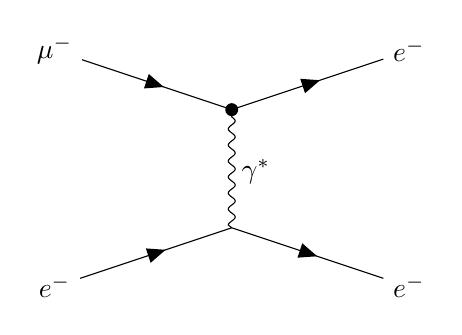
\begin{tikzpicture}[scale=0.75]
        \begin{feynman}

            \vertex (mu) at (-3,2) {\(\mu^-\)};
            \vertex (ei) at (-3,-2) {\(e^-\)};
            \vertex [dot] (v1) at (0,1) {};
            \coordinate (v2) at (0,-1) {};
            \vertex (e1) at (3,2) {\(e^-\)};
            \vertex (e2) at (3,-2) {\(e^-\)};

            \diagram* {
                (mu) -- [fermion] (v1) -- [fermion] (e1),
                (ei) -- [fermion] (v2) -- [fermion] (e2),
                (v1) -- [photon, edge label=\(\gamma^{*}\)] (v2),
            };

        \end{feynman}
        \end{tikzpicture}
        \caption{}
        \label{fig:photonic-direct}
    \end{subfigure}
    \hfill
    % (b) Photonic exchange interaction
    \begin{subfigure}[b]{0.32\textwidth}
        \centering
        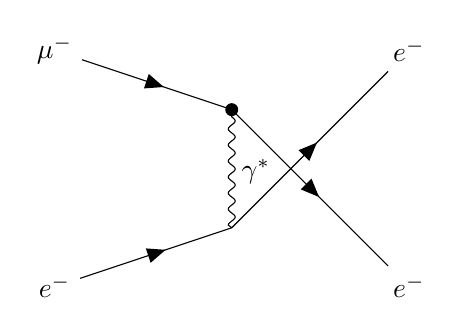
\begin{tikzpicture}[scale=0.75]
        \begin{feynman}

            \vertex (mu) at (-3,2) {\(\mu^-\)};
            \vertex (ei) at (-3,-2) {\(e^-\)};
            \vertex [dot] (v1) at (0,1) {};
            \coordinate (v2) at (0,-1) {};
            \vertex (e1) at (3,2) {\(e^-\)};
            \vertex (e2) at (3,-2) {\(e^-\)};

            \diagram* {
                (mu) -- [fermion] (v1) -- [fermion] (e2),
                (ei) -- [fermion] (v2) -- [fermion] (e1),
                (v1) -- [photon, edge label=\(\gamma^{*}\)] (v2),
            };

        \end{feynman}
        \end{tikzpicture}
        \caption{}
        \label{fig:photonic-exchange}
    \end{subfigure}
    \hfill
    % (c) Contact interaction
    \begin{subfigure}[b]{0.32\textwidth}
        \centering
        \begin{tikzpicture}[scale=0.75]
        \begin{feynman}

            \vertex (mu) at (-3,2) {\(\mu^-\)};
            \vertex (ei) at (-3,-2) {\(e^-\)};
            \vertex [dot] (v) at (0,0) {};
            \vertex (e1) at (3,2) {\(e^-\)};
            \vertex (e2) at (3,-2) {\(e^-\)};

            \diagram* {
                (mu) -- [fermion] (v) -- [fermion] (e2),
                (ei) -- [fermion] (v) -- [fermion] (e1),
            };

        \end{feynman}
        \end{tikzpicture}
        \caption{}
        \label{fig:contact-interaction}
    \end{subfigure}

    \caption{Tree-level Feynman diagrams contributing to
    $\mu^- e^- \to e^- e^-$ (a) direct photonic interaction,
    (b) photonic exchange interaction represented by the terms with $A_{\text{L,R}}$ and (c) four-fermion contact interaction represented by the $g_i$ terms. In each instance, the black dot represents a BSM vertex.}
    \label{fig:clfv-interaction-diagrams}
\end{figure}

In the paper here \cite{NewProcess2010}, the photonic interactions are discussed and the possible branching ratios in either a photonic-dominated ($A_{R,L}>>g_i$'s) or contact-dominated ($g_i >> A_{R,L}$) reality are discussed as well as possible rates and cross sections as functions of the coefficients for a selection of related processes to the $\muEtoEE$ process. Further, it is identified that the energy of the final state should reflect the initial state of a muon approximately at rest recoiling off of a nucleus. This approximately monoenergetic signature for both electrons at about half the muon rest mass is crucial in the identification of the process in experimental design (see \S~\ref{subsec:ExpSignature}).

Further calculation and analysis of the contact interactions are computed via nonrelativistic approaches and partial wave analysis in a follow-up paper \cite{ImprovedAnalyses2016} by Yuichi Uesaka, Yoshitaka Kuno, Joe Sato, Toru Sato, and Masato Yamanaka in 2016. It is important to note that in these papers that photonic and contact interactions can be distinguished based on the effects of atomic number $Z$ in the resulting Coulomb field processes. In this paper, the angular distribution and normalized differential templates for 
\begin{equation}\label{eqn:differentialTemplate}
    \frac{d^2\Gamma}{\Gamma \ dE \ d\cos\theta}
\end{equation}
are outlined and constrained with specific attention paid to affects in $^{208}\text{Pb}$ nuclei. These differential templates give the distribution of the angular dependence depending upon the recoil amount of the nucleus and gives an almost entirely back-to-back angular distribution. An example can be seen in the plot from the paper by Uesaka et all in the below figure \ref{fig:PbDifferentialTemplate} illustrating a relevant $g_1$ type interaction in a $^{208}\text{Pb}$ nucleus.

\begin{figure}[h!]
    \centering
    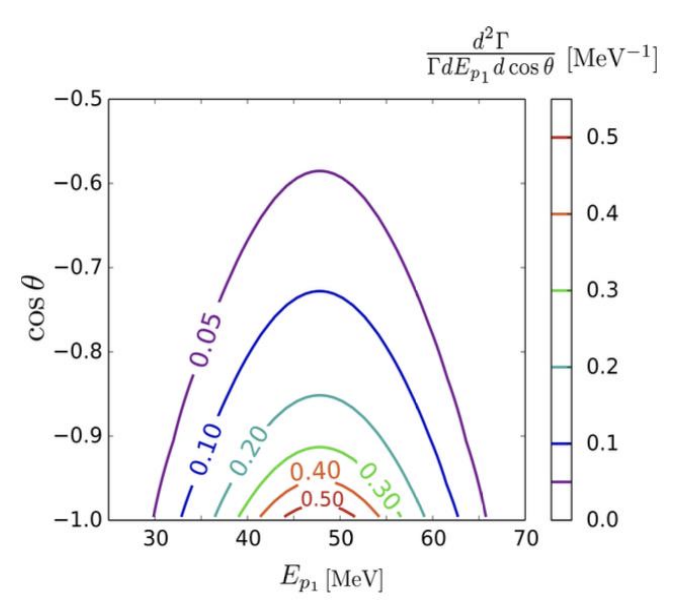
\includegraphics[width=0.5\linewidth]{Images/TheoryImages/PbDifferentialTemplate.png}
    \caption{The normalized double differential rate with respect to final state particle energy and angle shown as a level curve in cosine of opening angle, $\cos\theta$, and particle energy, $E_{p_1}$ for $^{208}\text{Pb}$ $g_1$ type interaction. The majority of the probability for the process appears approximately back-to-back and at approximately half the muon rest mass energy with decreasing probability further from this limit.}
    \label{fig:PbDifferentialTemplate}
\end{figure}

Theory points towards this process as a viable experimental channel to test given it's wide phase space and sensitivity to short and long lived mediators as well as variability in wave function overlap given variation of atomic number (charge). Especially active models that are being investigated by phenomenologists include axion-like particles and other short heavy lived mediators that may contribute to BSM physics. \cite{KumarPetrov2026MuonicAtoms} It is an investigation of this specific process in the Mu2e experiment that is the principle goal of this dissertation research proposal.

\subsection{Previous Tests of Charged Lepton Flavor Violation} \label{subsec:PreviousTests}

In the last 30 years there have been many experimental constraints placed on models describing flavor change. The majority of the limits were placed in $1998$ by SINDRUM II. However, given the new technology and collaborative efforts, improvements in the sensitivity of experiments can now allow further constraining of the models, or possibly detection! A table listing all the currently established limits can be seen in table \ref{tab:clfv_limits}.

\begin{table}[h!]
\centering
\caption{Current limits on selected charged lepton flavor violating processes. The process highlighted in yellow has not been directly tested; however, by crossing symmetry, its limit is inferred from the SINDRUM limit on $\mu^+ \to e^+e^-e^+$. Data are taken from the larger table in Calibbi and Signorelli (2018) \cite{CalibbiSignorelli2018CLFVIntro}.}
\label{tab:clfv_limits}
\begin{tabular}{l c c l c}
\hline
Reaction & Present limit & C.L. & Experiment & Year \\
\hline
$\mu^+ \to e^+\gamma$
& $< 4.2 \times 10^{-13}$ & 90\% & MEG at PSI & 2016 \\

$\mu^- \mathrm{Ti} \to e^- \mathrm{Ti}^{\dagger}$
& $< 6.1 \times 10^{-13}$ & 90\% & SINDRUM II & 1998 \\

$\mu^- \mathrm{Pb} \to e^- \mathrm{Pb}^{\dagger}$
& $< 4.6 \times 10^{-11}$ & 90\% & SINDRUM II & 1996 \\

$\mu^- \mathrm{Au} \to e^- \mathrm{Au}^{\dagger}$
& $< 7.0 \times 10^{-13}$ & 90\% & SINDRUM II & 2006 \\

$\mu^- \mathrm{Ti} \to e^+ \mathrm{Ca}^{*\dagger}$
& $< 3.6 \times 10^{-11}$ & 90\% & SINDRUM II & 1998 \\

$\mu^+e^- \to \mu^-e^+$
& $< 8.3 \times 10^{-11}$ & 90\% & SINDRUM & 1999 \\

$\tau \to e\gamma$
& $< 3.3 \times 10^{-8}$ & 90\% & BaBar & 2010 \\

$\tau \to \mu\gamma$
& $< 4.4 \times 10^{-8}$ & 90\% & BaBar & 2010 \\

$\tau \to eee$
& $< 2.7 \times 10^{-8}$ & 90\% & Belle & 2010 \\

$\tau \to \mu\mu\mu$
& $< 2.1 \times 10^{-8}$ & 90\% & Belle & 2010 \\

$\tau \to \pi^0e$
& $< 8.0 \times 10^{-8}$ & 90\% & Belle & 2007 \\

$\tau \to \pi^0\mu$
& $< 1.1 \times 10^{-7}$ & 90\% & BaBar & 2007 \\

$\tau \to \rho^0e$
& $< 1.8 \times 10^{-8}$ & 90\% & Belle & 2011 \\

$\tau \to \rho^0\mu$
& $< 1.2 \times 10^{-8}$ & 90\% & Belle & 2011 \\
\hline

$\mu^+ \to e^+e^-e^+$
& $< 1.0 \times 10^{-12}$ & 90\% & SINDRUM & 1988 \\

\rowcolor{yellow!25}
$\mu^-e^- \to e^-e^-$
& $< 1.0 \times 10^{-12}$ & 90\% & SINDRUM$^{*}$ & 1988 \\
\hline
\end{tabular}
\end{table}

The current limits set by the experiments shown in table \ref{tab:clfv_limits} demonstrate areas that can be improved with next generation detector systems, especially those at the intensity frontier of particle physics research. The Mu2e experiment, Mu3e, and other next generation experimental designs are looking for improvements to these sensitivities to further constrain theoretical models describing CLFV processes.
%================================================
% 2. Experimental Motivation and Signature
%================================================
\section{Experimental Motivation and Signature} \label{sec:ExpMotivAndSignature}
\subsection{Mu2e Primary Goal and Approach}\label{subsec:Mu2ePrimaryGoal}

The Mu2e Experiment serves as a powerful next generation investigation of charged lepton flavor violation (CLFV) in the intensity frontier. The primary goal of the Mu2e Experiment is to investigate the coherent conversion of a muon to an electron in the field of a nucleus, the process $\muToe$ in aluminum. Specifically, the Mu2e experiment looks to constrain (or measure) the branching ratio of the process by investigating 
\begin{equation}\label{eqn:Mu2eBranchingRatio}
    R = \frac{\mu^- N\to e^- N}{\text{all other muon decay channels}},
\end{equation}
hoping to improve upon the previous measurement made by SINDRUM II by four orders of magnitude \cite{Bernstein2019}.
This process signature is a monoenergetic ($104.973$ MeV/c), single reconstructed electron with viable background constraints in place via timing and detector construction. While this signal is quite clean, it requires a precise experimental construction to mediate any backgrounds that might misrepresent a signal process of interest. The most relevant background of interest in this proposal is that of muon decay-in-orbit (DIO) that results in the Standard Model permitted (primary) decay of $\mu^- \to e^- + \bar{\nu}_e + \nu_\mu$, which is a three body decay preserving lepton flavor. A full schematic representation of the Mu2e experiment can be seen in figure \ref{fig:Mu2eExperiment} and a thorough description of the experimental design detailing construction parameters, materials, tolerances, and background reduction procedure can be found in work by Bernstein in \cite{Bernstein2019} as well as the Mu2e Technical Design Report (TDR) \cite{Mu2eTDR}. 
\begin{figure}[h!]
    \centering
    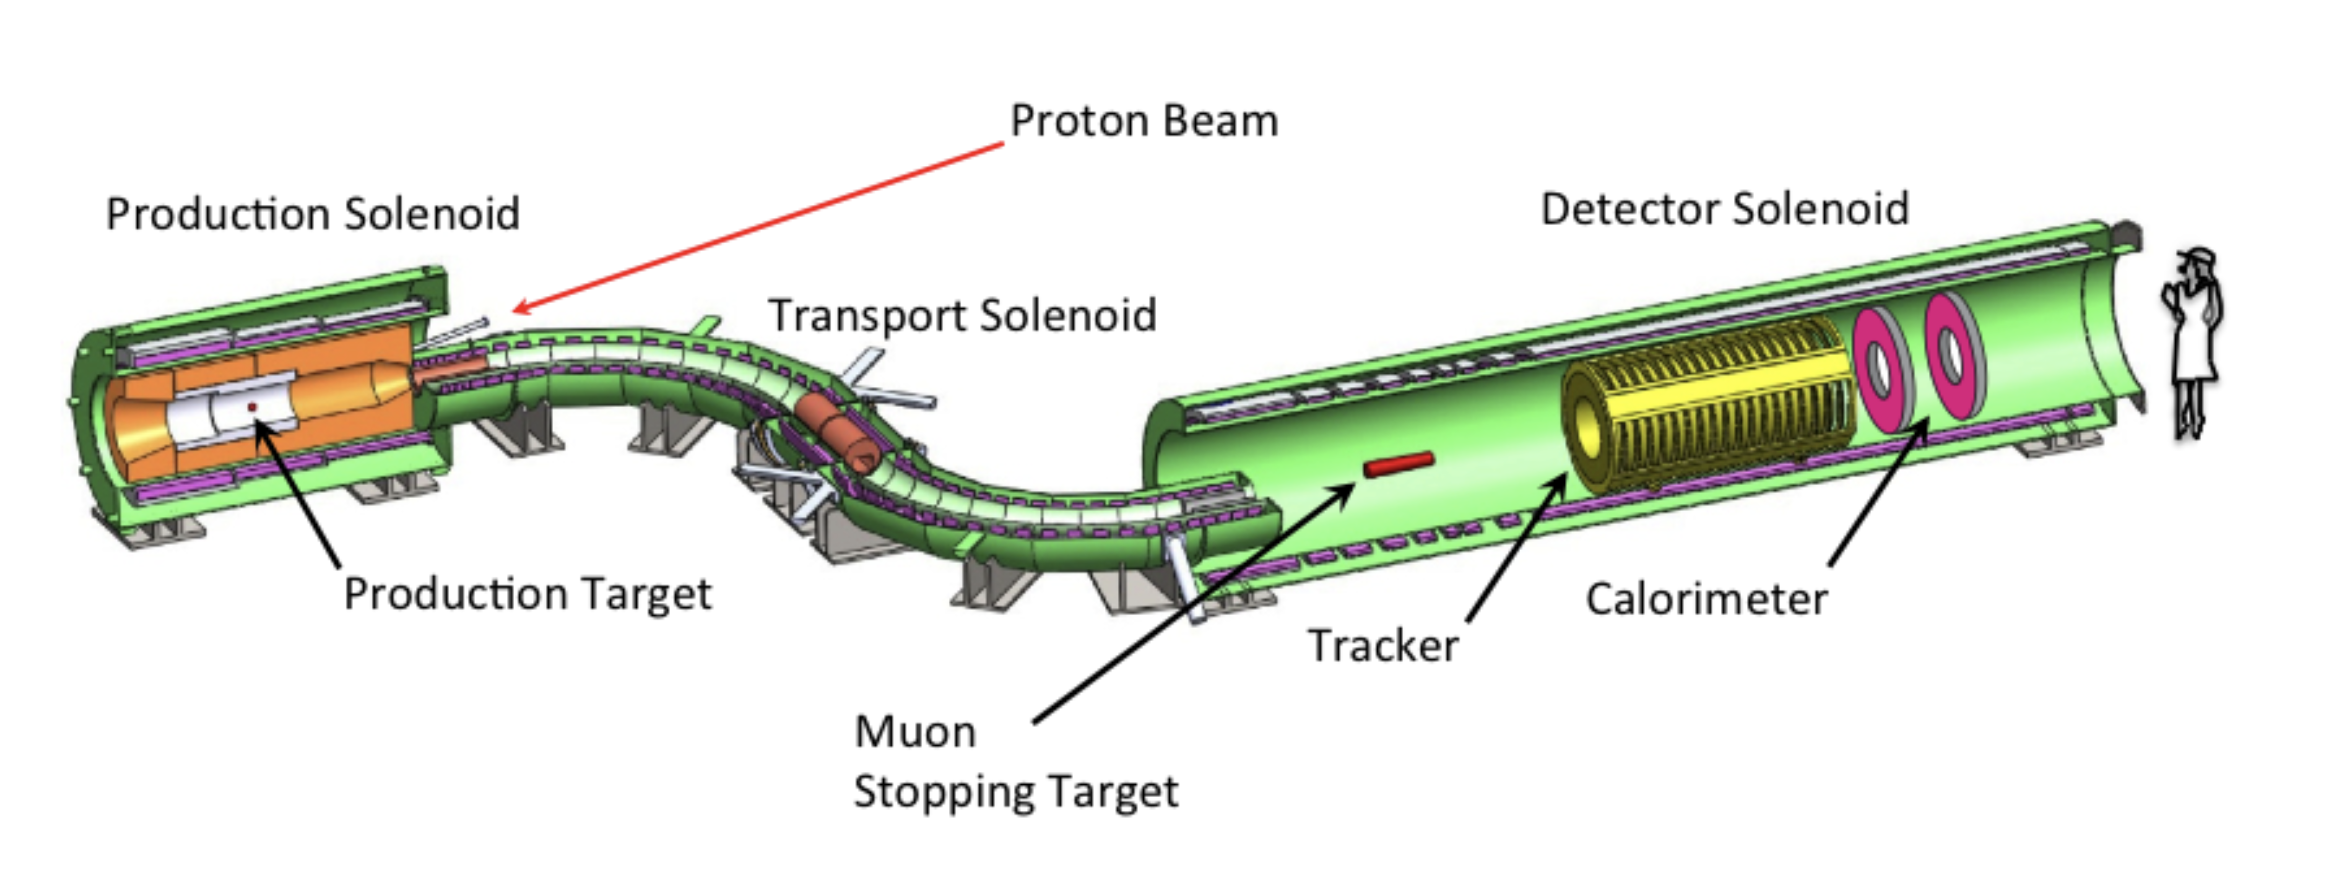
\includegraphics[scale=0.3]{Images/ExperimentImages/Schematics/Mu2eExperimentSchematic.png}
    \caption{A schematic view of the Mu2e Experiment with all essential components labeled.}
    \label{fig:Mu2eExperiment}
\end{figure}

\subsection{Experimental Signature of $\muEtoEE$ and Experimental Requirements in Mu2e} \label{subsec:SignatureMuEtoEE}

Given the large intensity of muons on target in the Mu2e Experiment, there are multiple other channels available for testing BSM physics and constraining models. The primary channel of interest for this proposal is that of $\muEtoEE$, a two-electron final state constrained in kinematics by energy and angular effects as discussed in \S~\ref{subsec:MuEtoEETheory}. 

For a muon decaying via this process, there are a few main signal characteristics that can be used to identify it in the Mu2e Experiment by its final state. In order to qualify as a final state of this process, the following conditions need to be met. There must be an identifiable pair of electrons of energy approximately equal to half the muon rest mass, The electrons must also be emitted approximately back-to-back from one another. Finally, there must be a reconstructible common origin vertex location and time for the process to occur. 
\begin{itemize}
    \item two reconstructed electrons in the final state
    \item electron energy of approximately half the muon rest mass ($E\approx m_\mu/2 = 52.8$ MeV/c)
    \item  emission of pair of electrons with approximately back-to-back angular separation
    \item common origin position and time
\end{itemize}

These characteristics make this process a very interesting and clean signal to look for in experimental designs. Most electromagnetic processes that may occur in a detector result in the emission of a positron and electron pair and/or a photon, so the two electron final state is a powerful differentiator given that they are of like charge rather than opposite. Further, the kinematic constraints of the final state mean that the majority of events containing a decay of this type can be identified if the orientation of the detector can put constraints on the angular emission of the pair. Finally, along with all the other signal characteristics, in the instance of a strong vertexing algorithm/software for reconstructed tracks, the final state is identifiable by a common origin position and time. This differentiates the final state from the possible mixing of other sources of electrons, most especially, multiple instances of Standard Model decay and decay-in-orbit electrons. 

While the signal is especially clean in general, in the Mu2e Experiment, there are specific requirements for measuring this channel that must be applied. In order to have the events be stored, a specialized trigger must be added that selects events of the signature of interest for analysis. Collaboration effort with the trigger group is required for this stage. Further, for both electrons at this energy to be visible in the detector system, the detector solenoid would need to be set at half-strength magnetic field still possessing the same magnetic field gradient mapping as the full field configuration. This ensures that the low momentum electrons in the $50$ MeV/c region will not be filtered through the annulus of the detector system and that the magnetic mirror effect still applies. However, given that this places the active region of the tracker in the path of the primary DIO background, so as to reduce deadtime and pileup, this also requires that the intensity be decreased by a significant fraction. The actual fraction remains to be calculated and simulated in the process of determining required run time. Finally, there needs to be implemented vertexing software in the computing environment to determine the common origin point. A detailed description of steps to be taken can be found in \S~\ref{sec:Proposal} in the proposal of the dissertation work to be done. 

%================================================
% 3. Preliminary Results
%================================================
\section{Initial Investigation} \label{sec:InitialInvestigation}

In order to determine the viability of generating and simulating a $\muEtoEE$ process in the Mu2e computing environment, preliminary tests were conducted in order to determine generator formation, signal survival through reconstruction, and rudimentary vertexing using reconstruction products. This section details the approaches taken as well as the results seen up to this point. 

\subsection{Monte Carlo Event Generator Development and Validation}\label{subsec:MCGenDevValid}

As stated in \S~\ref{subsec:SignatureMuEtoEE}, and in \S~\ref{subsec:MuEtoEETheory}, the $\muEtoEE$ process is notable in that it has a specific set of defining characteristics that make it a powerful candidate for checking different channels of CLFV in the Mu2e Experiment, namely the approximately monoenergetic distribution, the largely back-to-back angular distribution, and the common origin vertex. In order to determine if the pure process could potentially be seen, a toy generator was constructed that threw two electrons of the same energy entirely back-to-back with direction sampled randomly from a unit sphere. 

This toy generator called \verb|B2BCeEndpoint|, as the name implies, relies on alteration of the existing functional generator for the conversion electron generator that is used in the Mu2e collaboration for the conversion process of interest $\muToe$. The changes that were made to the existing \verb|CeEndpoint| generator created a second instance of the conversion electron produced with its initial momentum direction exactly 180 degrees opposite from the original instance and changed th energy to approximately half the muon rest mass. Further, it was also necessary to create supporting code in the Production workflow to ensure that this generator was able to be used in the Mu2e Computing environment. Notable adjustments include creating a FHiCL file to be used in the primary generation stage corresponding to this process and addition of our channel to coded list of all identified generators so that the correct process code can be identified in the Monte Carlo truth. 

The actual system of event generation here is the construction of a custom instance of the Mu2e structure \verb|art::EDProducer| module to generate the two-electron state that would be thrown in the back-to-back orientation. Part of the implementation of the module requires the use of a FHiCL input to be given to select stopping target material, input particles, pdg, and verbosity of the process. The module reads a collection of simulated muons from earlier up the chain called a \verb|SimParticleCollection| containing simulated $\mu^-$ particles stopped in the aluminum stopping target. Then from there, the module identifies eligible muons and selects one parent muon to be the location of the process occurrence. Two daughter electrons are created at the location of the parent muon, and they are thrown in a back-to-back orientation with energy of 
$$
E_1 = E_2 = \frac{m_\mu}{2}.
$$
These events are thrown from the random assortment of muons according to the decay by a random exponential dependent upon the material-dependent muon half life $\tau_\mu$

$$
f(\Delta t)=\frac{1}{\tau_\mu}e^{-\Delta t/\tau_\mu}.
$$
For some random direction selected from a unit sphere called $\hat{\mathbf{n}}$, we produce our momenta to be $\mathbf{p}_1=p\,\hat{\mathbf{n}}$ and $\mathbf{p}_2=-p\,\hat{\mathbf{n}}$ where the magnitude of the momentum vector is defined by 
$$p=\sqrt{E_i^2-m_\mu^2}$$
where $E_i$ is the energy of the $i$-th electron in the final state. This allows us to construct a Lorentz four-vector object to add to the output \verb|SimParticleCollection| for each of the two particles originating from the muon stops of the forms
$$
p_1^\mu = (E_1,\mathbf{p}_1) \ \ \ \text{and} \ \ \ p_2^\mu = (E_2,\mathbf{p}_2).
$$
These four-momenta along with particle type, process code, parent muon, and origin time (from global time) are stored in the output and run through the digitization and reconstruction stages of the simulation. 

In order to ensure that the thrown particles were constructed correctly (i.e. back-to-back with the correct energy) the momentum components were printed out to the terminal once the particles were generated. These console outputs could be then read and plotted to histograms for validation sake. Uniformity can be seen in the figure \ref{fig:gen_testAngularDependenceFullKinematics}
\begin{figure}[h!]
    \centering
    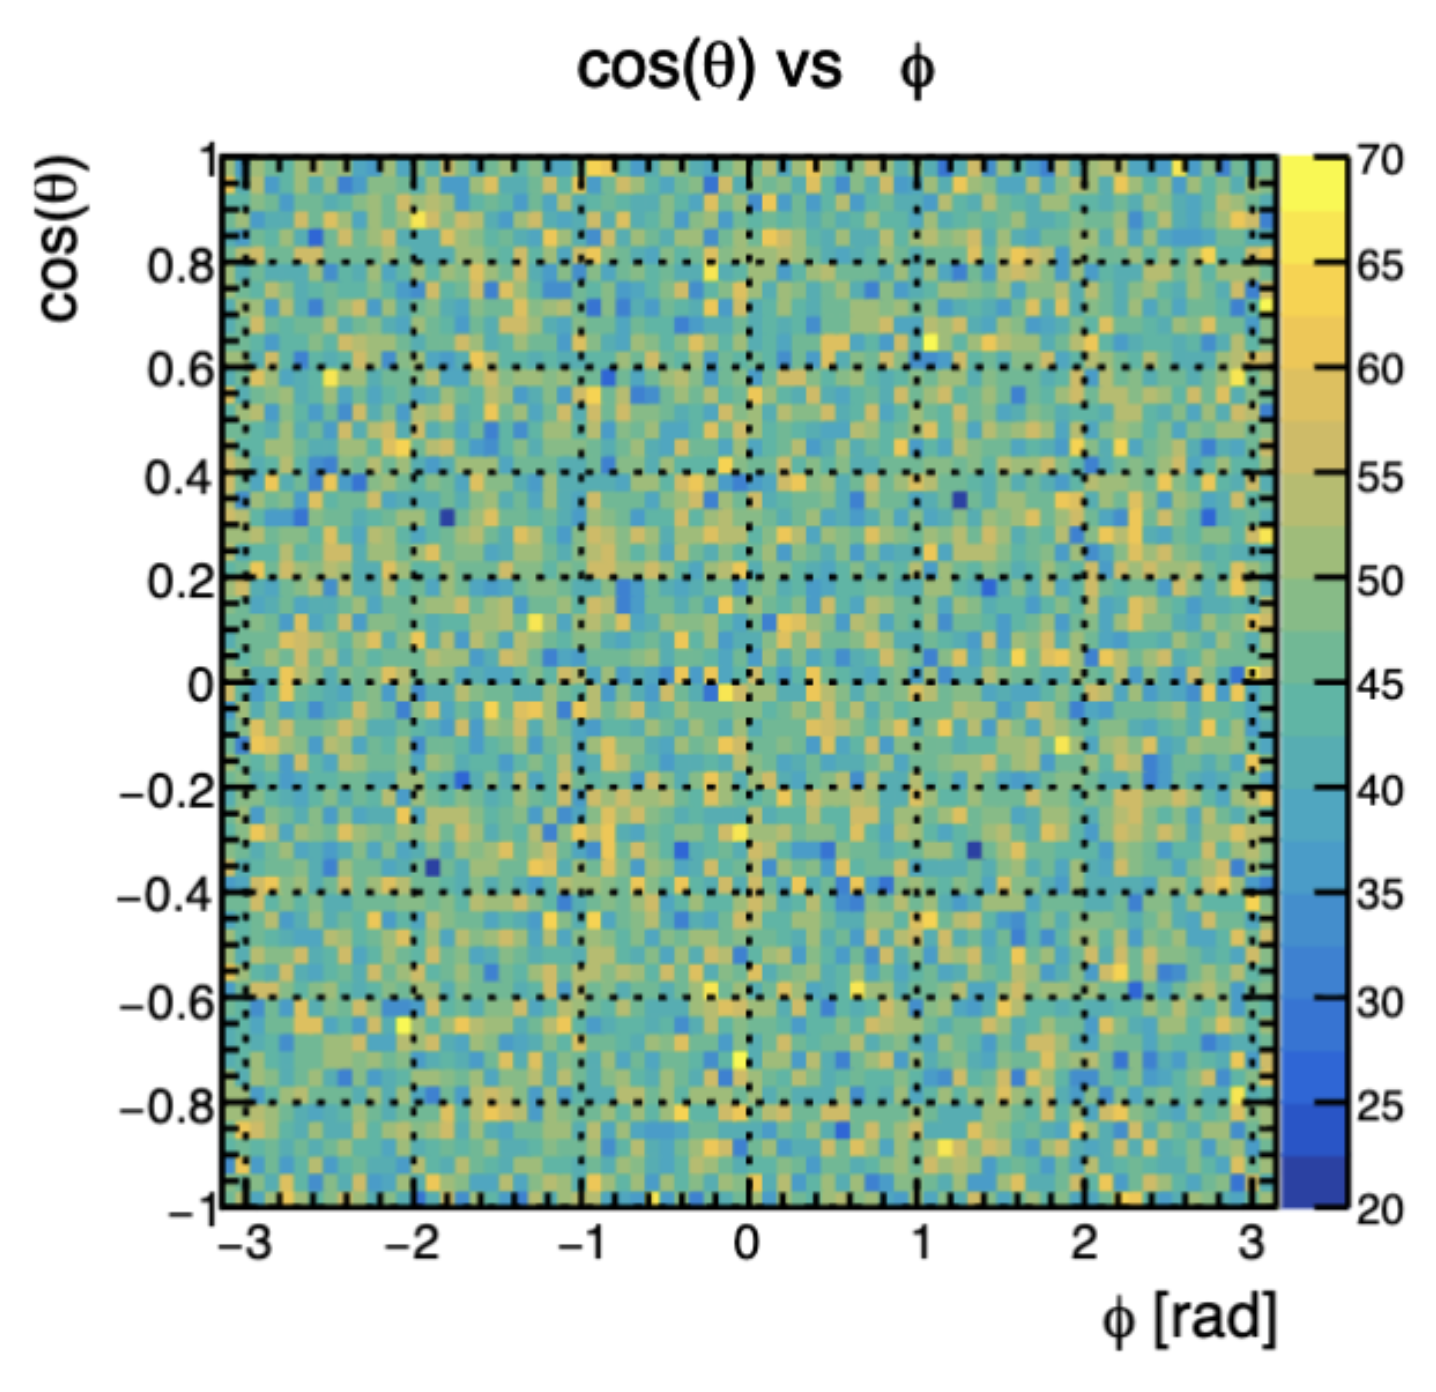
\includegraphics[scale=0.2]{Images/GeneratorTestImages/GenTest_HundredThousandAngularDist.png}
    \caption{Angular distribution of the momentum vectors thrown in the generator prior to any cuts. Illustrates uniformity across all of space.}
    \label{fig:gen_testAngularDependenceFullKinematics}
\end{figure}
The back-to-back nature can be seen from figure \ref{fig:gen_testThetaTheta}
\begin{figure}[h!]
    \centering
    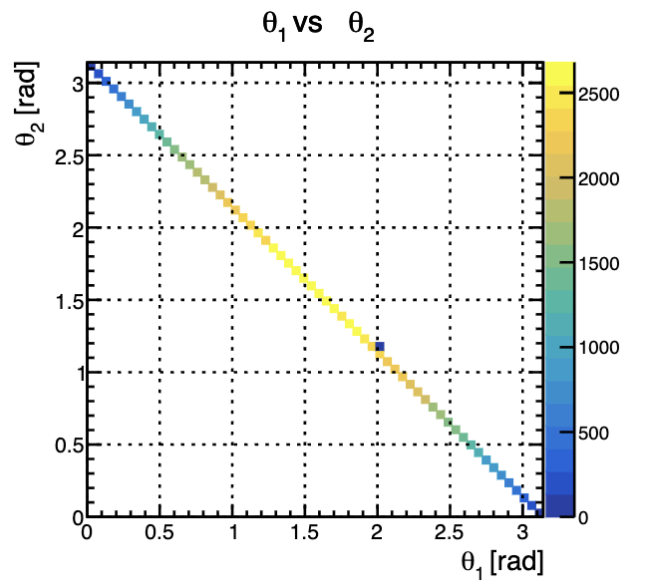
\includegraphics[scale=0.5]{Images/GeneratorTestImages/GenTest_HundredThousandThetaThetaPlot.png}
    \caption{Two dimensional histogram showing theta of the momentum from one thrown electron ($\theta_1$) versus the momentum of the other electron ($\theta_2$). A linear relationship with negative slope can be seen as expected.}
    \label{fig:gen_testThetaTheta}
\end{figure}
In order to show that the momentum magnitude is correct, a third plot was generated and can be seen in figure \ref{fig:gen_testMCMomMagnitude}
\begin{figure}[h!]
    \centering
    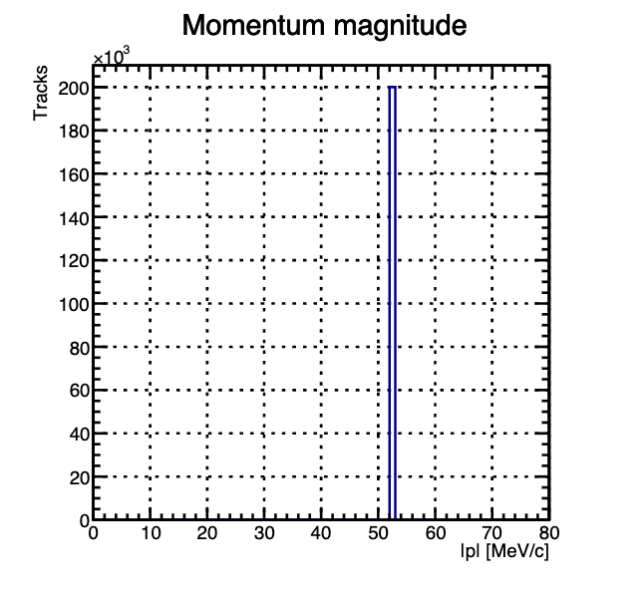
\includegraphics[scale=0.5]{Images/GeneratorTestImages/GenTest_HundredThousandMCTruthMom.png}
    \caption{A histogram illustrating a single valued peak of momentum magnitude at the desired value reaching a count of 200,000 tracks, as expected from 100,000 thrown electrons in the generator.}
    \label{fig:gen_testMCMomMagnitude}
\end{figure}

These three plots serve as validation of the intended kinematics of the desired generator. 

\subsection{Analysis Products from Stops in the Pure-Toy Generator Workflow} \label{subsec:AnalysisProductsPure}
Once the generator has been shown to produce the desired results, it needs to be actually utilized in the simulation of the experiment. The pure back-to-back process was run through the simulation workflow in the Mu2e computing environment beginning with throwing the one-hundred thousand generated process events from the muon stops in the aluminum target. The standard procedure starting from this stage is to run a simulation through the stages here:
\begin{equation}\label{eqn:workflowSteps}
    \text{Primary Generation} \to \text{Digitization} \to \text{Reconstruction} \to \text{Ntuple-Construction}
\end{equation}
Primary generation represents the simulation of the actual physics process that is being thrown towards the detector including the collision with detector components and influence by ambient fields and components, taking into account the geometric acceptance of the detector system. From here, the effects of the byproducts of the physics processes of interest that are incident upon detector components are simulated in the digitization process. These simulated digitized products of process interactions with detector components are then utilized in a reconstruction formalism using kinematic Kalman (KinKal) fitting techniques developed by Dave Brown for the Mu2e Collaboration to attempt to determine the parameterizations and trajectories taken by particles of various types that could be moving through the detector in different directions. For a more thorough background of the process of KinKal fitting, see \cite{Brown2024KinKal} where a full description is described for the three types of trajectories and the motivation for this approach versus standard fitting procedures is discussed. From there, all the relevant analysis structures are compiled into a more manageable package called an Ntuple, which can then be analyzed using basic CERN ROOT tools and scripts.

Running the full physics simulation of the process and the detector response allows a user to determine the functionality of the generator itself as well as determine specific cuts that can be made to isolate signals of interest. In this process, the 100,000 events were simulated from muon stops for the pure back-to-back kinematics generator and the resulting ntuple was analyzed. 

Analysis of the resulting data product ntuple 

Utilizing the Mu2e collaboration's event visualization tool called \verb|EventDisplay|, figure \ref{fig:EventDisplay2TrackEvent} illustrates the Monte Carlo truth of an example event simulated up through the reconstruction phase. 

\begin{figure}[h!]
    \centering
    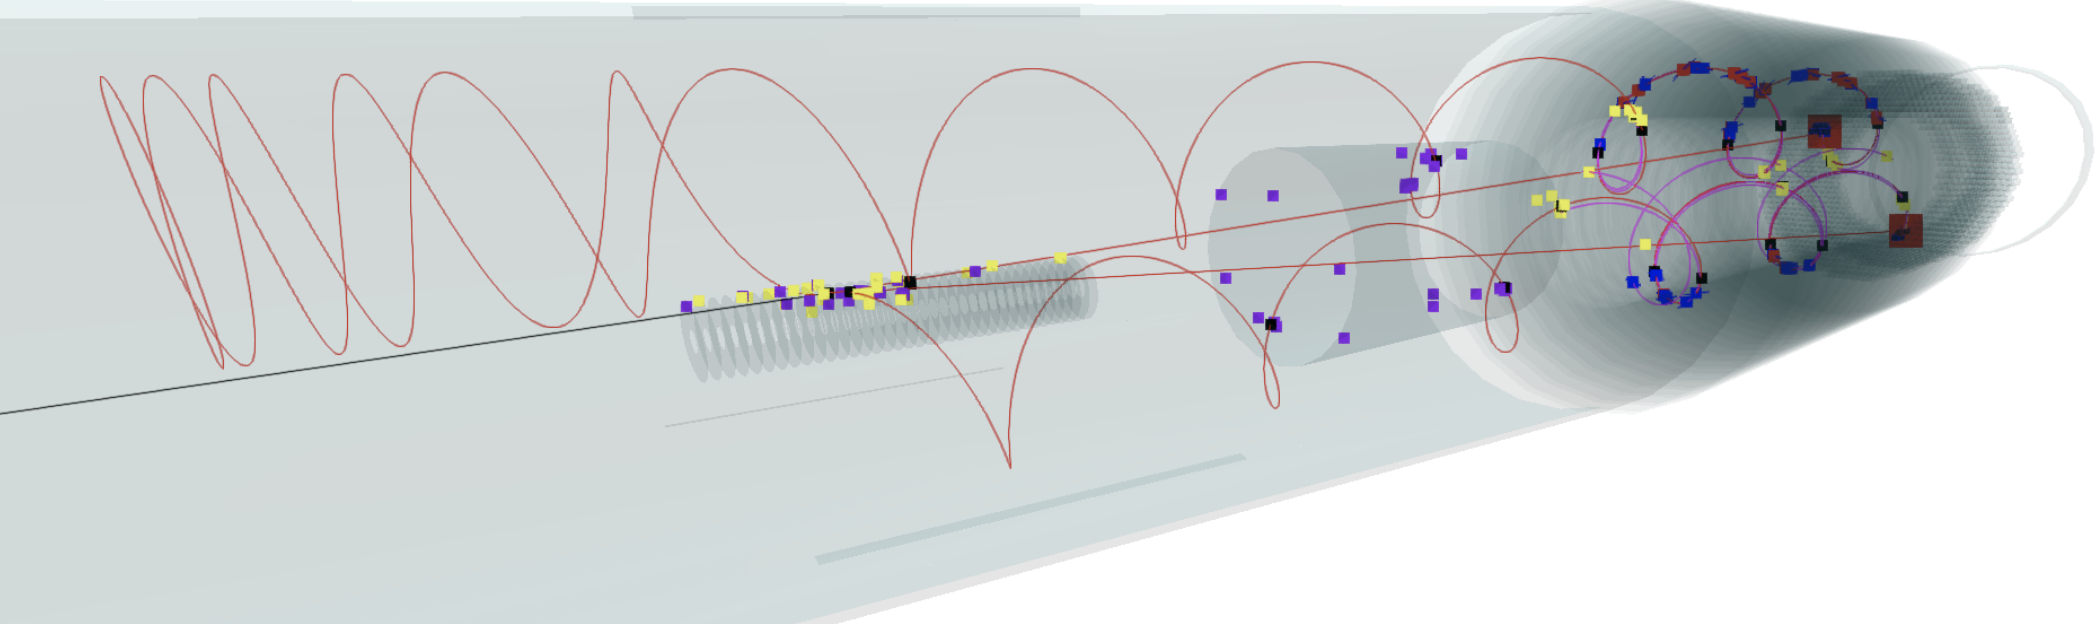
\includegraphics[scale=0.4]{Images/ExperimentImages/Data/EventDisplayTwoTrackEvent.png}
    \caption{The Monte Carlo truth trajectory helices of a two track back-to-back electron event that survived the simulation through reconstruction emitted from one of the stopping target foils. In the case of the backwards going electron track, there is a very obvious affect due magnetic field gradient in the simulated detector solenoid, a so-called "Magnetic Mirror effect." Two calorimeter hits are apparent in the red squares at the far end of the detector system.}
    \label{fig:EventDisplay2TrackEvent}
\end{figure}

\subsection{Candidacy Cuts for Vertexing}\label{subsec:VertexingCuts}

For the sake of creating a selection criteria for signal discrimination, three stages of cuts were applied to events that made it the full way through the reconstruction stage. 

The first cut was to limit the number of reconstructed tracks to be exactly two. Events with less than two tracks are not able to be discriminated from decay-in-orbit events, which are monoenergetic in the same energy regime as the process of interest. Further, events with more than two tracks at this stage are very rare (only consisting of six total events) given that this is a pure process. In further stages of this sensitivity study where background processes are mixed in, more refined techniques for discrimination of higher track numbers will need to be developed and implemented. However, at this stage simply cutting the noise for identifying the most pure signal is adequate.  

The second cut was that a "good" calorimeter hit was required for both tracks in a given event. In the reconstruction process, a "good" calorimeter hit identifies that an adequate amount of energy was deposited into the calorimeter cluster in order to designate it as active in the digitization process. This also means that the termination of the trajectory must be identified as either the front or the rear calorimeter disk. In selecting only events in which the calorimeter is activated, this provides discrimination for the Kalman fitter and also can be used to constrain angular separation of tracks in the signal selection criteria. The specifics of the angular constraint on the calorimeter hits will be investigated in later stages of the sensitivity study to determine viability.

The final cut constrained the momentum of the final state to be within $50-53 \text{ MeV/c}$. Give the propagation of ionization, Bremsstrahlung, and other electromagnetic process electrons in the detector final states, this type of cut makes it easy to differentiate the process (which sits at a higher energy) than these processes while also giving room for energy loss as the final state electrons pass through material. This cut was applied last in order to ensure that noise was not being included in the subsequent vertexing process. 

Table \ref{tab:event_survival} illustrates the cuts being made after each stage of simulation as well as after each signal discrimination cut, \ref{tab:event_survival}. It can be seem from the table that after all cuts are made, there is over a $16.7\%$ efficiency in a pure-process sample. 
\begin{table}[htbp]
\centering
\caption{Event survival through the reconstruction and selection chain.}
\label{tab:event_survival}

\begin{tabular}{|c|c|c|}
\hline
\textbf{Process} & \textbf{Surviving Events} & \textbf{\% of Total} \\
\hline
Muon Stops & 100,000 & 100\% \\
\hline
Surviving Primaries & 66,545 & 66.545\% \\
\hline
Digitization & 50,792 & 50.792\% \\
\hline
Reconstruction & 50,792 & 50.792\% \\
\hline
Exactly Two Track Reconstruction & 31,221 & 31.221\% \\
\hline
Good Calo Hit for Each Track & 23,253 & 23.253\% \\
\hline
Momentum Cut ($50$--$53~\mathrm{MeV}/c$) & 16,771 & 16.771\% \\
\hline
\textbf{Final Candidates} & 16,771 & 16.771\% \\
\hline
\end{tabular}
\end{table}

From these cuts, the histograms of the momenta of the surviving reconstructed tracks (at tracker middle) can be plotted alongside the Monte Carlo truth momenta as can be seen in the figure \ref{fig:RecoMomCutProgression_AllCutsAndMCTruth}.

\begin{figure}[h!]
    \centering
    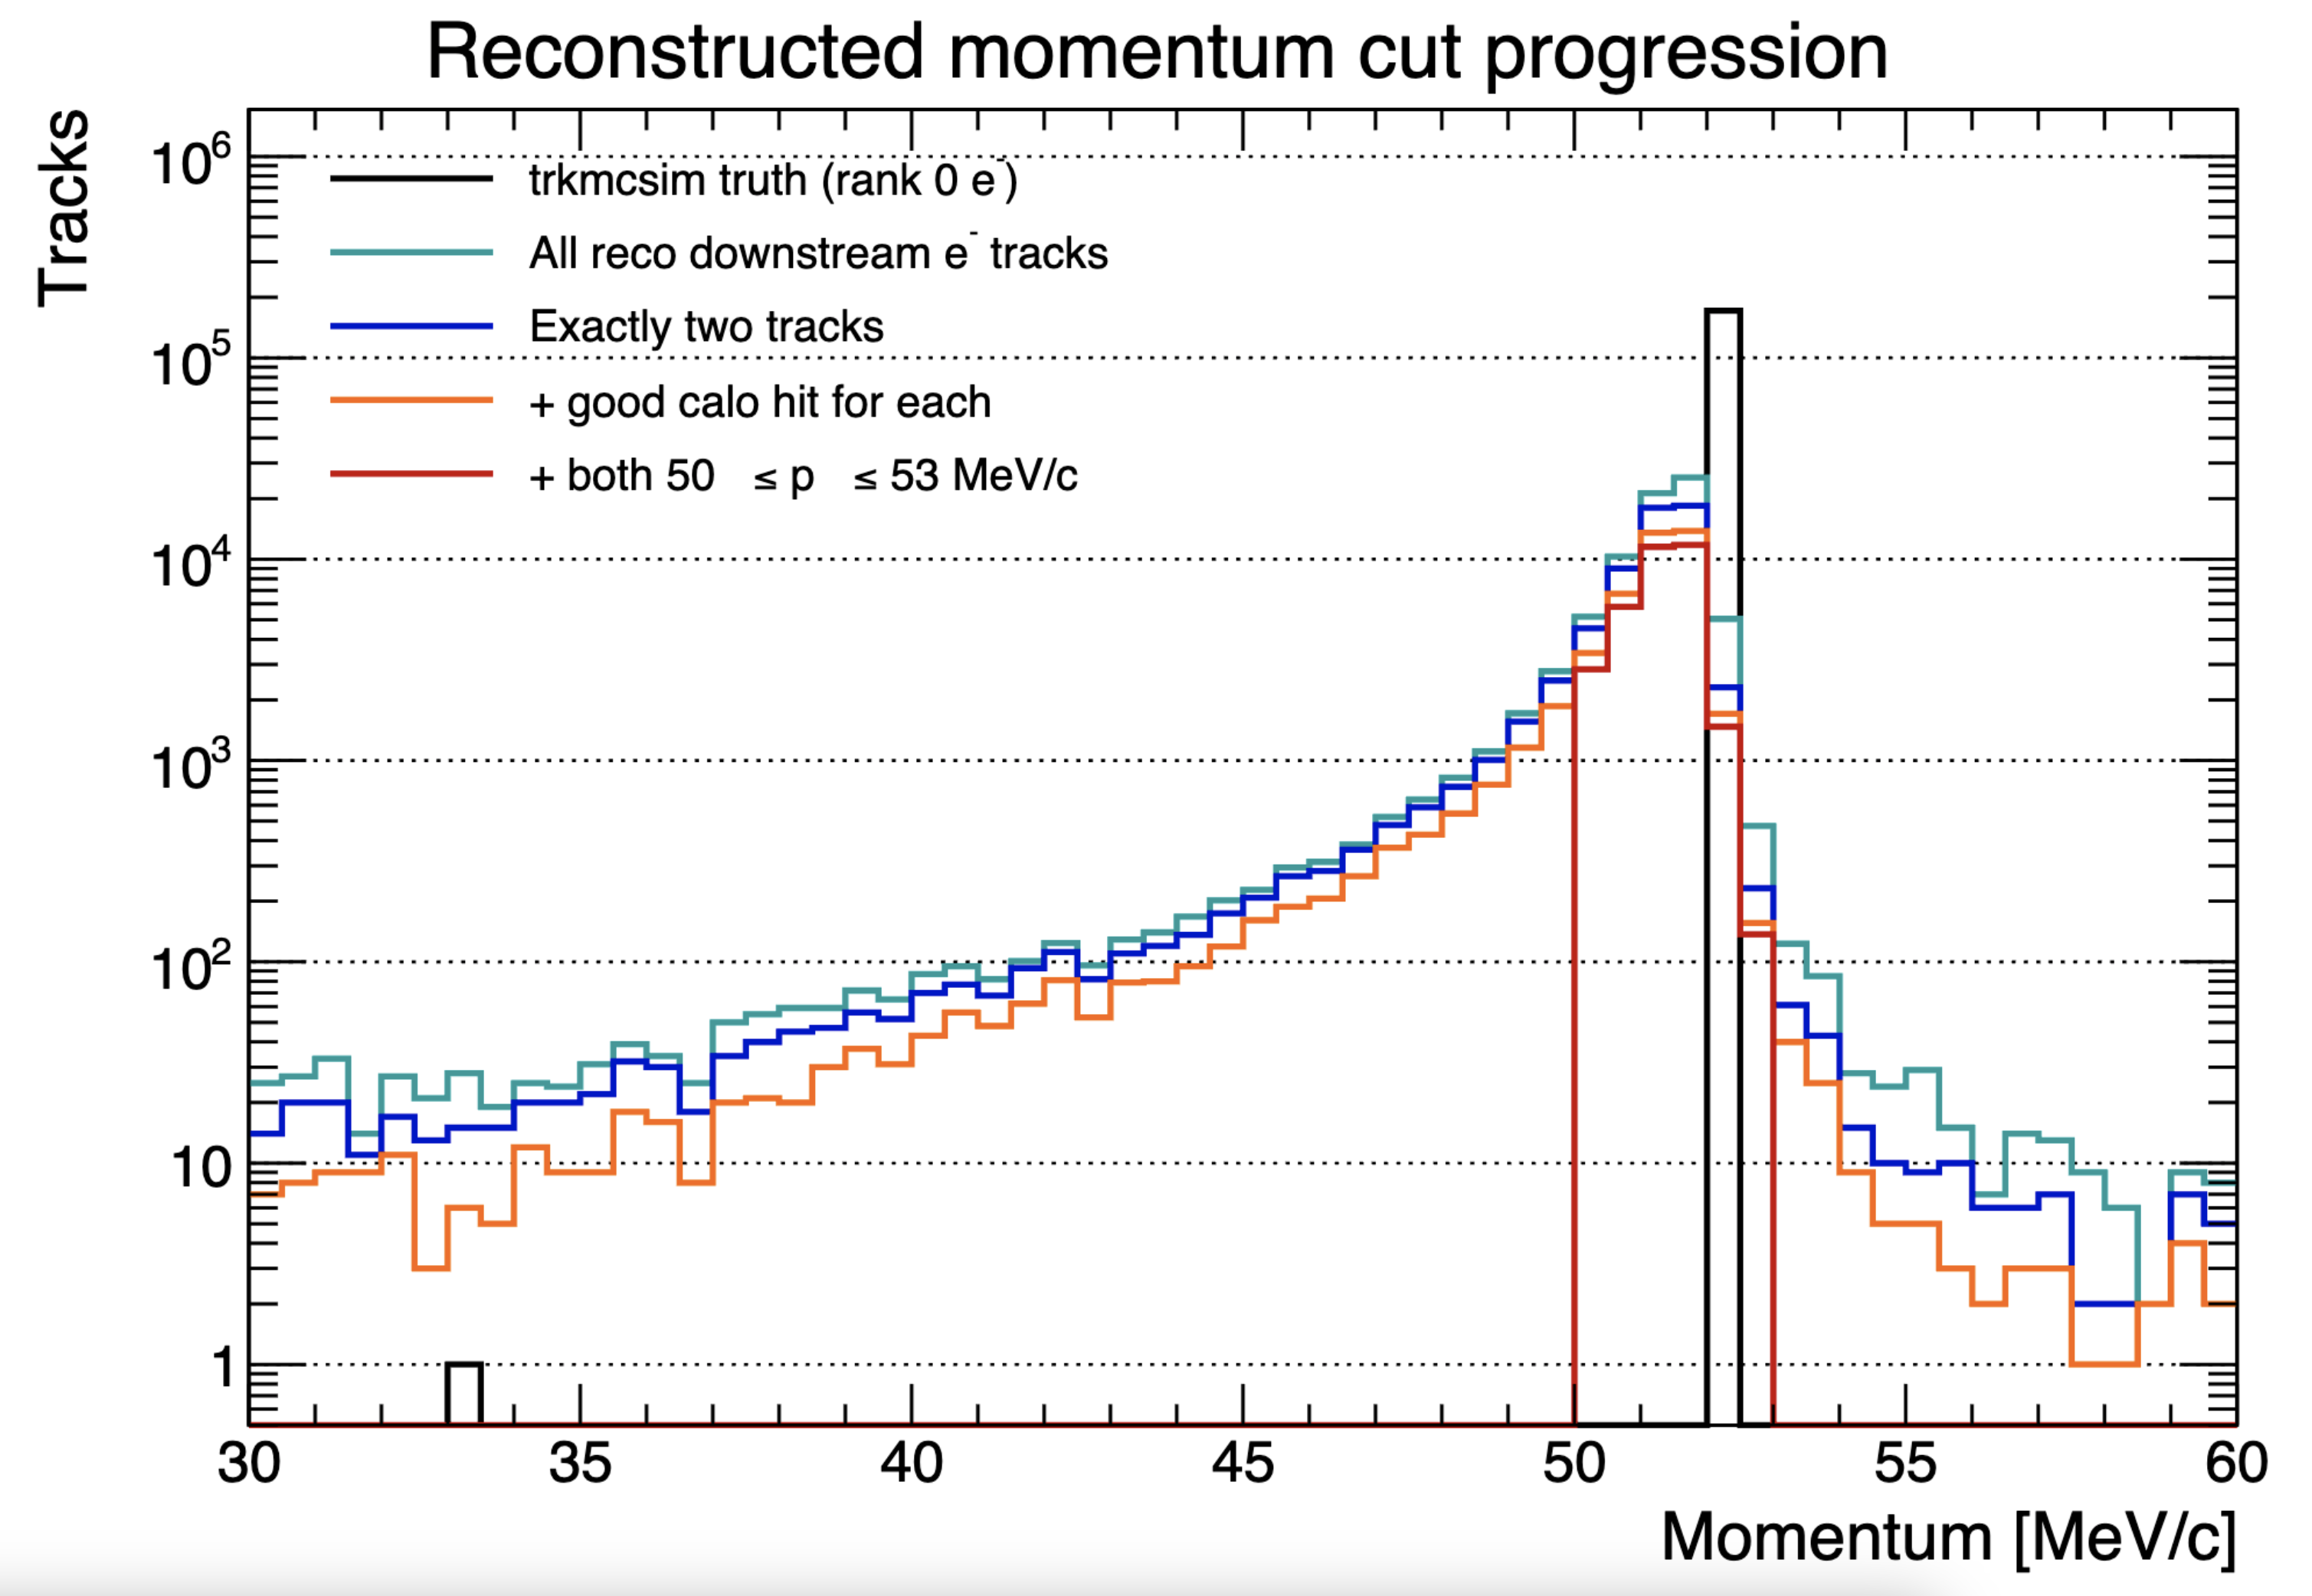
\includegraphics[scale=0.25]{Images/TrkSegsImages/AuxillaryReco/RecoTrackSegmentMomentumOverlay_AllCutsAndMCTruth.png}
    \caption{Momentum histogram representing the progression of cuts made for candidate electron tracks. Count axis displayed in logarithmic coordinates and final candidate electron tracks taken after all cuts made (red plot).}
    \label{fig:RecoMomCutProgression_AllCutsAndMCTruth}
\end{figure}

While the generator threw the momenta for the 100,000 events in a uniform complete solid angle, the surviving event tracks did not cover the complete solid angle in Monte Carlo Truth.As can be seen by figure \ref{fig:MCTruthSurvivingRecoTracks}, when the momentum angles at the origin position for rank zero (process selected) electrons, there is a smaller angular distribution that is allowed in the polar angle for electron tracks that make it the entire way through reconstruction. The azimuthal angle remains uniform. The polar angle maximum for this sample is $128.1^\circ$ and the minimum is $32.7^\circ$.

\begin{figure}[h!]
    \centering
    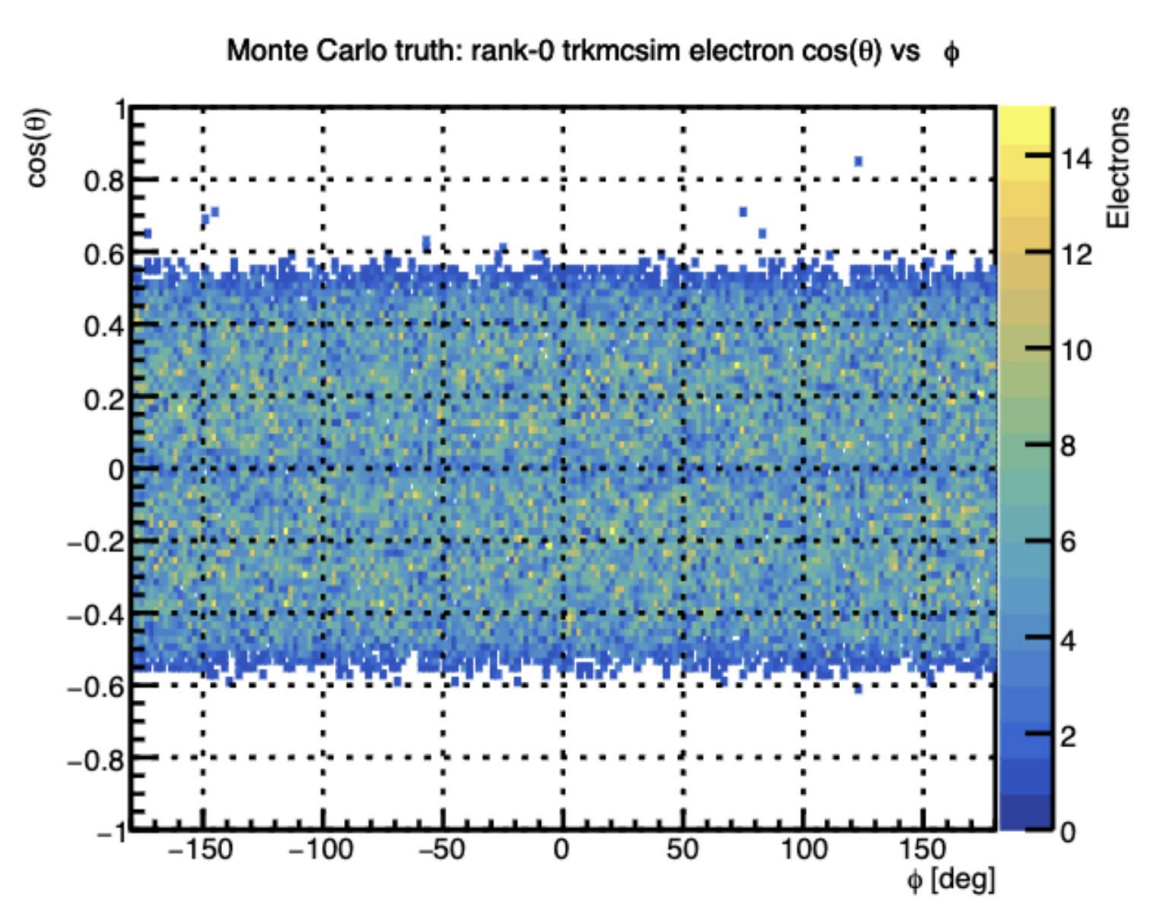
\includegraphics[width=0.5\linewidth]{Images/ExperimentImages/Data/MonteCarloTruthSurvivingReconstructedTracks.png}
    \caption{Angular distribution of the Monte Carlo truth momentum for rank-0 electrons. The maximum and minimum angles as collected are at $\theta=128.1^\circ$ and $\theta = 32.7^\circ$ respectively.}
    \label{fig:MCTruthSurvivingRecoTracks}
\end{figure}

The simulation of the pure back-to-back, half energy generator in the Mu2e computing environment produced ample analyzable data products that can be investigated in various ways. Not only are the data products holding readable information, but also, that information can be used to draw conclusions about origin position to be analyzed in comparison with the Monte Carlo truth in the development of new vertexing software for the Mu2e computing system.

\subsection{Vertexer Development and Validation} \label{subsec:VertexerDev}

In order to determine the ability to generate a common reconstruction vertex using analysis data structure (n-tuples), a rudimentary vertexing methodology was implemented on pure-process datasets generated in the Mu2e simulation environment. After our selection cuts, we employed the following rudimentary procedure for predicting a common origin of tracks.

Each track that is reconstructed in the Mu2e computing environment is plotted as it passes through various surfaces in the detector system. These intersections for selected surfaces such as middle of the tracker, inner proton absorber and stopping target foils are stored inside the n-tuple structures as track segments (trksegs). Each trkseg has intersections with a given surface and is given a position $\vec{r}_0$ and momentum $\vec{p}$ where they intersect the surface. Tracks are selected according to shared intersection with a particular stopping foil. Should two tracks share more than one foil of intersection, then the foil intersection with the smallest time parameter separation between the predicted intersection points is selected. Each of the two tracks selected in each event were parameterized linearly (according to some common origin in the reconstruction) as

\begin{equation}
\mathbf{r}_1(s) = \mathbf{r}_{1,0} + s\,\hat{\mathbf{p}}_1, \ \ \ \text{and} \ \ \  \mathbf{r}_2(t) = \mathbf{r}_{2,0} + t\,\hat{\mathbf{p}}_2,
\end{equation}

where $\vec{r}_{i,0}$ details the intersection position through a selected surface and $\hat{p}_{i}$ is the unit vector in the direction of the $i$th reconstructed track's momentum at that given pair of points along these parameterizations. It is worth noting that given the fact that $\hat{\mathbf{p}}_1$ and $\hat{\mathbf{p}}_2$ are both unit vectors defined without units, we must have that $[t]=[s]=\text{mm}$, as we need these parameters in units of length. We can define a distance vector between them as
$$
\mathbf{D}(t,s) = \mathbf{r}_2(t) - \mathbf{r}_1(s) = \mathbf{r}_{2,0} - \mathbf{r}_{1,0} +t\,\hat{\mathbf{p}}_2 - s\,\hat{\mathbf{p}}_1 = \mathbf{w}_0 +t\,\hat{\mathbf{p}}_2 - s\,\hat{\mathbf{p}}_1
$$
where $\mathbf{w}_0$ is defined as the difference in the origin positions for convenience. Because we have a distance vector we can find the distance between any two points by taking the magnitude as
$$
\left|\mathbf{D}(t,s)\right| = \sqrt{|\mathbf{w}_0|^2+t^2+s^2+2t\,\mathbf{w_0}\cdot\hat{\mathbf{p}}_2-2s\, \mathbf{w}_0\cdot\hat{\mathbf{p}}_1-2ts\,\hat{\mathbf{p}}_1\cdot\hat{\mathbf{p}}_2}.
$$
To find the distance of closest  approach, we want to minimize this function, or, given the fact that $|\mathbf{D}(t,s)| \geq 0$ for all $t,s\in \mathbb{R}$, minimize the function $F(t,s)= |\mathbf{D}(t,s)|^2$. To do so, we need to find the values $s^*$ and $t^*$ such that
$$
\frac{\partial F}{\partial s} = 0 \ \ \ \text{and} \ \ \ \frac{\partial F}{\partial t} = 0.
$$
This gives us the coupled system of equations
\begin{align*}
    \frac{\partial F}{\partial s} &= 2s - 2\left(\mathbf{w}_0\cdot\hat{\mathbf{p}}_2\right)-2t\left(\hat{\mathbf{p}}_1\cdot\hat{\mathbf{p}}_2\right) = 0 \\
    \frac{\partial F}{\partial t} &= 2t +2\left(\mathbf{w}_0\cdot\hat{\mathbf{p}}_2 \right)-2s\left(\hat{\mathbf{p}}_1\cdot \hat{\mathbf{p}}_2\right) = 0
\end{align*}
These equations give us the closest approach parameters of
\begin{equation}\label{eqn:closestSValue}
    s^* = \frac{\left(\mathbf{w}_0\cdot\hat{\mathbf{p}}_1\right)-\left(\hat{\mathbf{p}}_1\cdot\hat{\mathbf{p}}_2\right)\left(\mathbf{w}_0\cdot\hat{\mathbf{p}}_2\right)}{1-\left(\hat{\mathbf{p}}_1\cdot\hat{\mathbf{p}}_2\right)^2}
\end{equation}
and 
\begin{equation}\label{eqn:closestTValue}
t^*=\frac{\left(\mathbf{w}_0\cdot\hat{\mathbf{p}}_1\right)\left(\hat{\mathbf{p}}_1\cdot\hat{\mathbf{p}}_2\right)-\left(\mathbf{w}_0\cdot\hat{\mathbf{p}}_2\right)}{1-\left(\hat{\mathbf{p}}_1\cdot\hat{\mathbf{p}}_2\right)^2}.
\end{equation}
A more geometric approach can be used to find the same equations for $t^*$ and $s^*$ and is detailed in appendix \ref{app:GeoParameters} relying upon the cross product of the unit vectors and how it relates to the distance between the two lines for any given parameters $t$ and $s$.

On these two lines we identify the parametric vectors for the points of closest approach called $\mathbf{r}_1(s^*)$ and $\mathbf{r}_2(t^*)$ where the $*$ represents the particular parameter value that gives the closest approach as seen below
$$
\mathbf{r}_1(s^*)= \mathbf{r}_{1,0} + s^*\hat{\mathbf{p}}_1 \ \ \ \text{and} \ \ \ \mathbf{r}_2(t^*) = \mathbf{r}_{2,0}+t^* \hat{\mathbf{p}}_2
$$

and can be calculated by utilizing those values found in equation \ref{eqn:closestSValue} and \ref{eqn:closestTValue}. From these vectors, we can identify a separation vector between these two by taking the difference
$$
\mathbf{D^*} = \mathbf{r}_2(t^*) - \mathbf{r}_1(s^*)
$$
with the spatial separation between the two being the magnitude 
$$
D^*=\left| \mathbf{r}_2(t^*) - \mathbf{r}_1(s^*)\right|.
$$
Assuming an almost equal momentum at production, we can foresee that a vertex should lie at the midpoint of this separation, a location that we can call 
\begin{equation}
    \mathbf{r}_{V} = \frac{1}{2}\left[\mathbf{r}_2(t^*)-\mathbf{r}_1(s^*)\right].
\end{equation}\label{eqn:vertexLocation}
A drawn image of this process can be found in figure \ref{fig:drawn_vertexer_algorithm}.
\begin{figure}[h!]
    \centering
    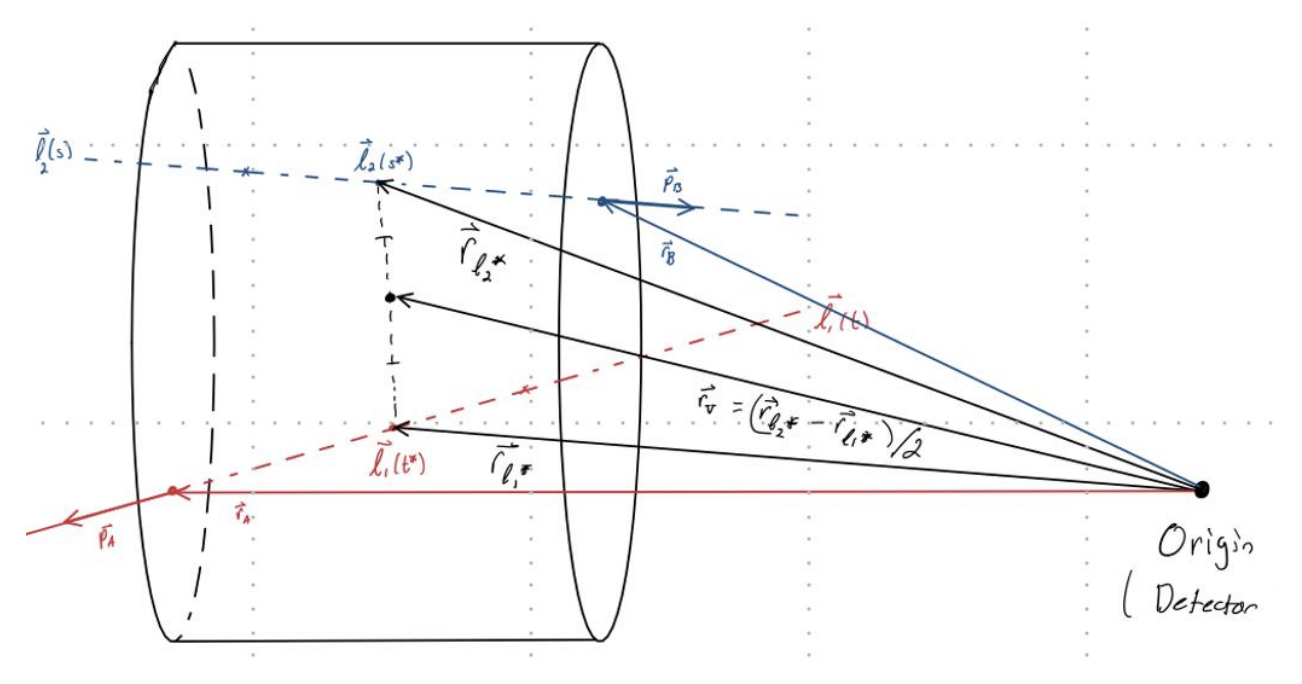
\includegraphics[width=0.5\linewidth]{Images/TrkSegsImages/Vertexer/Vertexer_Drawn.png}
    \caption{Illustration of the linear vertexing process. Linear parameterizations are shown as dotted lines through the intersection points along the momentum directions. Points are shown with the $*$'ed parameters. Vertex labeled at the center of the separation vector between these two points. All vectors are shown to be with reference to some detector origin configured in the simulation geometry.}
    \label{fig:drawn_vertexer_algorithm}
\end{figure}

This vertex created from the KinKal fit intersections contains three spatial components which can be plotted and compared to the stopping target dimensions. This process has been done for the small sample size as can be seen in figure \ref{fig:Vertexer_2D_Histograms}. It can be seen inside this figure that the $x,y$ and $x,z$ histograms are plotted with the majority of the vertices lying inside the dimensions of the stopping target.  

\begin{figure}[h!]
    \centering
    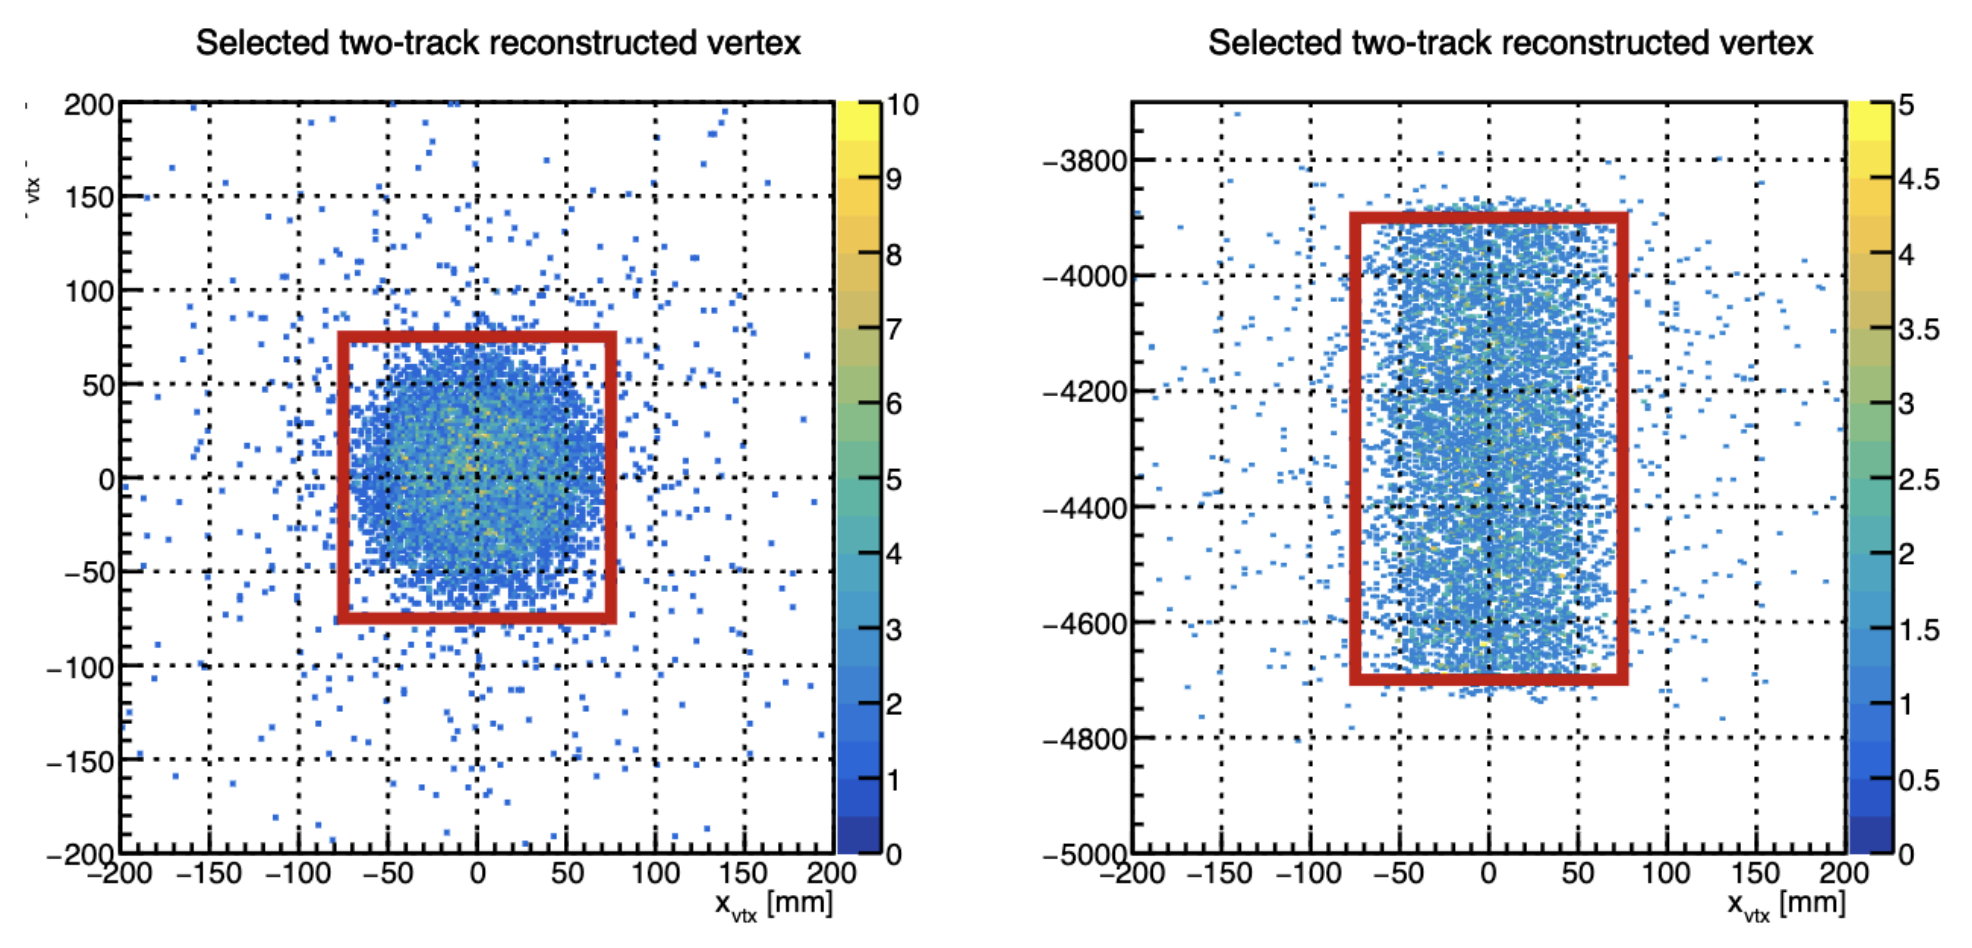
\includegraphics[scale=0.4]{Images/TrkSegsImages/Vertexer/Vertexer_2D_Histograms.png}
    \caption{2D Histogram of the reconstructed vertex locations for the linear extrapolation of reconstruction intersection positions and momenta in the stopping target. The stopping target dimensions are identified by the red boxes. Left figure shows the $x,y$ histogram while the right figure shows the $x,z$ histogram. The majority of reconstructed vertices are located inside the confines of the stopping target, however the inner annulus and the foil separations.}
    \label{fig:Vertexer_2D_Histograms}
\end{figure}

When one compares the position of the reconstructed vertex with the Monte Carlo truth origin position for the process of interest, a resolution is obtained. In the figure \ref{fig:Vertexer_resolutions_xyzr}, the resolution in $x$, $y$, $z$, and $r$ is computed. It can be seen in the resolution graphs that the $x$ and $y$ resolutions are fairly centralized with nominally small standard deviations. However, the $z$ resolution is quite problematic, being both largely off center, positively skewed, and having large standard deviation. This in turn greatly affects the resolution of $r$, the total distance magnitude between the two.

\begin{figure}[h!]
    \centering
    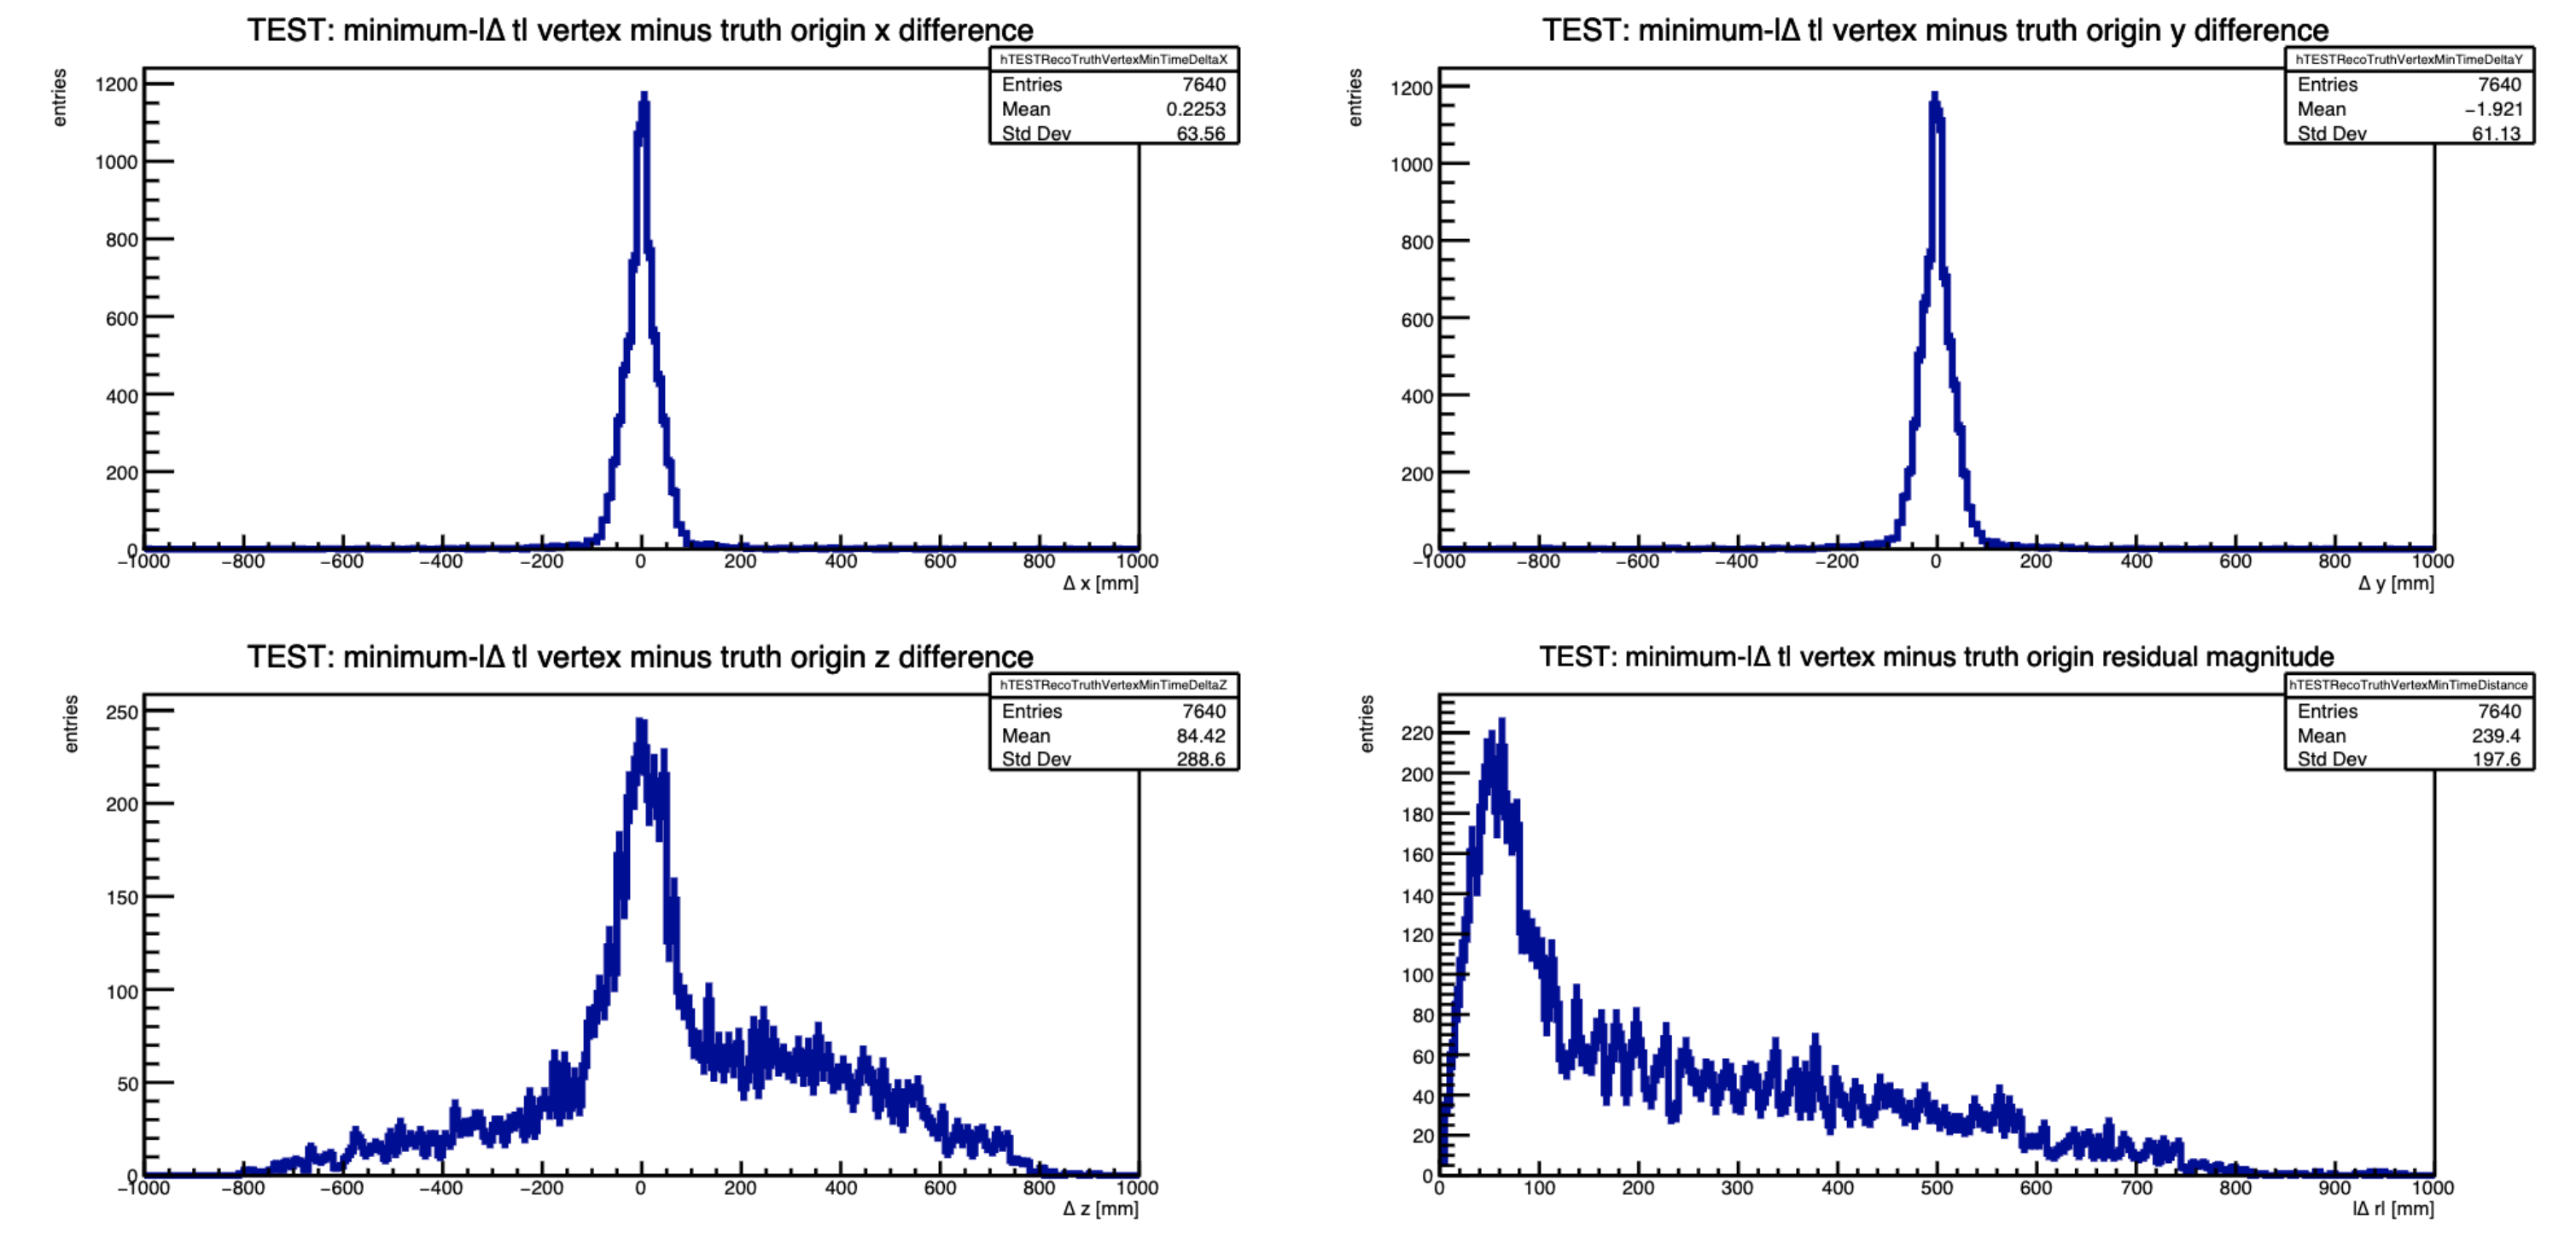
\includegraphics[scale =0.3]{Images/TrkSegsImages/Vertexer/Vertexer_XYZR_Resolution.png}
    \caption{Resolution plots of the difference between reconstructed vertex location and Monte Carlo truth origin position in the $x,y,z$ coordinates as well as total distance $r$. The $x,y$ resolutions are fairly stable, however, the $z$ resolution has problems.}
    \label{fig:Vertexer_resolutions_xyzr}
\end{figure}


While these results do demonstrate capabilities to formulate a generator in the Mu2e enviornment and beginning steps have been made to create a formal event signature, it is important to note the simplifications that have been employed in these initial stages. 

First, it must be addressed that the generator process being simulated does not exactly represent the theoretically predicted dynamics and kinematics expected for the $\muEtoEE$ process in aluminum. A very important challenge to overcome in the development of a true generator for this process is to find a closed form expression for the normalized double differential conversion rate with respect to the energy and angle as noted in equation \ref{eqn:differentialTemplate}. Such a calculation will be completed by a fellow PhD candidate at the University of South Carolina, Sudheer Muhammad, under the direction of Dr. Alexey Petrov. It is the derivation of this differential template for the different types of interaction that will be used as the theoretical basis for the generator angular and energy distribution probabilities that will be randomly sampled from.

Further, the vertexing procedure simplifies by utilizing parsed data and linear extrapolation and fitting. There are several issues that may contribute to the inability to formulate a well constrained vertex. The first (and largest concern) is that the intersection points stored inside the ntuple are not robust enough on their own to form a good prediction. The ntuple data structure is formulated from a reconstruction level data structure called an \verb|mcs.__.art| file. This art data product is a very dense and rich structure comprised of many TTrees from which the ntuple pulls its relevant information. Inside this \verb|mcs.__.art| file, there is more detailed descriptions of the parameterization of the particle trajectories and as a result, perhaps these parameterization details can be used to form a more consistent and accurate parameterization and thus reconstructed vertex. Given that in the current model, the construction is linear, the parameterization does not account for the helical nature of the paths as they move in the magnetic field. While the thickness of the foils are thin, a small adjustment such as moving from linear to helical trajectories could improve the resolution of origin location. Finally, there could be more aggressive cuts and constraints necessary to find strong vertex candidates that may have to be employed. Such constraints could be on the final state angles incident upon the calorimeter, specific numbers of foils hit, timing differences, or maximum number of backwards predicted reconstruction tracks. All of these additional cuts and any additional ones that arise in pattern analysis will be considered in the development of more precise vertexing programs to predict the true origin location and time of a process event.

Despite these simplifications made, the initial investigations have served as strong evidence that the $\muEtoEE$ channel can server as an interesting and important alternative CLFV channel in the Mu2e Experiment. This investigation and a formal, robust, high statistics sensitivity study for the $\muEtoEE$ channel in the Mu2e Experiment is the purpose of the proposed research goals and approaches below.

%================================================
% 4. Proposed Work
%================================================
\section{Proposed Work}\label{sec:Proposal}

The investigation work up to this point serves as a set of stepping stones to build a a full scale sensitivity study of the $\muEtoEE$ process in the Mu2e experiment. This section will illustrate some of the anticipated goals of such an undertaking, a list of actionable goals to achieve these goals to make a meaningful measurement, and a timeline of achievement of these goals.

\subsection{Dissertation Goals and Deliverables to be Completed and Collected} \label{subsec:Goals}

The primary research goal of this dissertation is: \textbf{produce a full, statistically sound sensitivity estimate of the $\muEtoEE$ process in the Mu2e experiment.} Following the investigative work done thus far, the following major progress goals and deliverables have been identified as important in the completion of this goal. In order to complete the dissertation work, these goals  can be broken up further into sub-goals for the purpose of thoroughly answering the needed research questions. This section serves to list the main objectives of the upcoming research work and establish the components that will contribute to the completion of those objectives.

\begin{enumerate}
    \item \label{goal:VertexImprovements}The first priority of the research will be to \textbf{generalize, formalize, and improve the vertexing procedure for the process based on more robust reconstruction products}. The common origin position and time is a critical signal identification characteristic without which the channel is indiscernible from backgrounds. Eliminating the simplifications is a reasonable starting point for the adjustments to the vertexer. Improvement of the vertexing software only aids in the event identification of the $\muEtoEE$ process and in generalizing the tool, can be used  to inform any multi-body final state analysis that may appear in the Mu2e experiment on a broader scale. Important stages to the completion of this goal in the pure process data files involve:
\begin{itemize}
    \item Investigate the various trees stored inside the \verb|mcs.__.art| data structure to identify stored helices and parameterizations along with covariance matrices for a more rigorous procedure.
    \item Utilize (or create) helical parameterization objects to find common origin positions and identify characteristics of import to the behavior of these parameterizations that may assist in event identification.
    \item Create a script to build an analyzable ntuple-like structure for specific vertexing and relevant data storage of pertinent "helix analysis data" using the art and FHiCL interface in the Mu2e computing system. This should be a similar container structure as ntuples for multi-track final state process analysis.
\end{itemize}
\textit{Deliverables for goal \ref{goal:VertexImprovements}:} Mu2e analyzable helix data structure and vertexing module developed and integrated into production/analysis workflow for relevant processes. Technical paper detailing the vertexing implementation in the Mu2e Experiment as well as an internal note detailing the use of the system.

\item \label{goal:Mixing}The next priority is to \textbf{create a mixed data sample of the back-to-back generator with relevant backgrounds.} The channel of interest is not the only process (and not the most prominent one) to exist inside the detector system during a configured run. To account for this, the pure process must be mixed with the relevant backgrounds. This goal will be completed in stages in order to determine the obscuring effects of each considered background and then compiled together for a full sensitivity prediction. The principle background is the muon decay-in-orbit that produces the Michel spectrum peaked at the energy level of our desired process. Other backgrounds that could influence the signal resolution include the cosmic ray background, radiative muon/pion capture as well as beam noise. The mixing process requires complicated scripts run to form large datasets in the computing grid, and thus, the core production team will be consulted regarding the appropriate procedure for this phase of analysis. 

All this being said, no sensitivity study would be complete without a thorough, layered analysis of the influence of different backgrounds and a full background study of the process of interest. The supporting steps to achieving this goal are
\begin{itemize}
\item investigate the primary backgrounds (DIO, cosmic, RPC, RMC, beam noise, etc.) as they interact with the $\muEtoEE$ process individually. This is immensely important for DIO specifically, as the pileup produced in the simulation at half field must be adequately tested in order to determine required intensity reduction of the incident protons on target.
\item overlap multiple backgrounds and scale them according to their influence on the ability to see the signal.
\item create a more robust signal identification discrimination process. Once mixing occurs, improved discrimination of large numbers of track per event will need to be investigated as well in order to make selections between similarities between process tracks and background tracks that appear in the same event. Background tracks, especially those DIO electrons will possess energy that can appear to be the same as the signal electrons. As a result, more sophisticated techniques and constraints for eliminating nonsense tracks will have to be utilized to prevent obfuscation of process tracks in an event or misidentification. Such tools could rely on implementations to specific configurations of the trigger, further identification of signal characteristics in different detector components (calorimeter, tracker, extra-detector scintillation), or even angular dependence in the calorimeter. A possible avenue that may be employed is the implementation of artificial intelligence or machine-learning (AI/ML) tools trained on specific process identification criteria.
\item perform statistical analysis to determine the required number of verified signal events to obtain significance or the number of incident protons on target (and thus, wall-clock hours) needed to surpass the constraints set by SINDRUM previous limit of similar processes as well as direct measurement
\end{itemize}
\textit{Deliverables for goal \ref{goal:Mixing}:} Analyzable simulation data set of pure and mixed process. A robust track discrimination process can be implemented for the process in the Mu2e computing environment. A proposal can be put out to the Mu2e collaboration for specific configuration runs at half-field in the active running stages depending on results.

\item \label{goal:theoryGenUpdate}The third priority is \textbf{implementation of true theoretical differential templates that account for nuclear recoil in the aluminum stopping target at high statistics.} As stated above at the end of \S~ \ref{sec:InitialInvestigation}, the generator does not account for the full kinematics of the process of interest and just throws electrons back-to-back at a prescribed energy of half the muon rest mass. The calculation of the differential templates described in equation \ref{eqn:differentialTemplate} for the $\muEtoEE$ process in an aluminum stopping target requires input from the collaborating theorists. The calculation should yield corrections to the energy and angular distribution of the thrown electrons similar to the figure shown for the $g_1$ type $^{208}\text{Pb}$ and as such, the photonic and contact term interactions must be calculated for the given atomic number $Z=13$ utilizing nonrelativistic partial wave approaches. Even being agnostic to the true physics, assuming that the decrease in $Z$ does not significantly impact the back-to-back nature and energy spectrum, the generator improvement would improve the accuracy of the predictions made of the mixed sample, especially at high statistics. Necessary details in the progression to this goal involve:
\begin{itemize}
    \item Derivation of closed form differential distribution functions to sample from in the generator stages for various interaction structures (photonic and contact) for the $\muEtoEE$ conversion in the presence of aluminum nuclei (completed by phenomenologist collaborators Sudheer Muhammad and Alexey Petrov at the University of South Carolina) using nonrelativistic field theoretic and partial wave approaches
    \item Calculation of relative probabilities of types of interaction based on available phase space (completed by phenomenologist collaborators Sudheer Muhammad and Alexey Petrov at the University of South Carolina).
    \item Creation of a generator correctly implemented into the Mu2e Offline computing environment  that accurately throws events based on the predicted weights of angular distribution and energy content of final state electrons (to be completed by Andrew Boldy)
    \item Simulation of the full $\muEtoEE$ generator in the Production workflow of the Mu2e simulation system at high statistics 
\end{itemize}
\textit{Deliverables for goal \ref{goal:theoryGenUpdate}:} Mu2e generator for the full $\muEtoEE$ process in the Mu2e experiment stopping target and a technical paper written alongside contributing theorists detailing the generator construction, implementation and theoretical background. An internal note for the Mu2e collaboration detailing the creation and use of the new generator as well as the sampling process.
 
 \item \label{goal:MLImplementation}Following the implementation of the full generator, the plan is to \textbf{create, train, and implement machine learning (ML) tools in the anomaly detection process for flagging background-inconsistent events and statistical analysis.} Given some amount of background processes, the $\muEtoEE$ process should appear as an unusual event signature (anomaly) in the data collected under particular running conditions and in simulations. One such area that can be investigated is the origin position difference between tracks in a multi-track event. The use of ML in the detection of anomalous signals in particle physics is an up-and-coming practice with versatility in the large data analysis and signal discrimination space \cite{MLAnomalyDetectionParticlePhysics2023}, but poses many additional requirements in order to implement it appropriately:
 \begin{itemize}
    \item Collect and analyze combined background simulation sample files to investigate the properties and simulations of these pure background processes and determine common characteristics/appearances amongst events in this sample.
     \item Identify characteristics to contribute to an anomaly-absent event feature vector $\mathbf{x}$ that also would be measurable in an anomalous event. These will store signal characteristics for both final state electrons as well as interactions with backgrounds and running conditions, $c$, in which the detector needs to be configured for the specific event characteristics. These features should come strictly from reconstructed/measured products, absent of Monte Carlo truth. The complete nominal signal that would occur in the simulation under configuration conditions $c$ should appear as a mixture of backgrounds, where the mixture is defined by a density
     \begin{equation}\label{DensityFunction}
     p_B(\mathbf{x}|c)=\sum_k \pi_k(c) p_k (\mathbf{x}|c)
     \end{equation} 
     where the $k$'s enumerate the background classes (DIO, cosmics, etc), $\pi_k$'s are the associated weights given a class such that their sum is equal to one, and the $p_k$'s are the probabilities of an event $k$ to produce features $\mathbf{x}$ under conditions $c$. 
     \item Create a machine learning model (neural-net, specifically) utilizing popular compatible code bases in the Mu2e computing environment, namely Python (PyTorch, scikit-learn, and/or TensorFlow) or C++ (LibTorch or the TensorFlow C++ API). The choice of model building environment depends on the integration capabilities within Mu2e computing and grid usage for following steps.
     \item Train the neural net on background data alone to establish a baseline structure for event feature vectors. For ease of implementation, training methodology for simulation could be supervised (including labels of process in the background) or self-supervised (process labels being determined by data). Both approaches should be done in order to validate the approach for Monte Carlo data as well as real-run data.
     \item Test the neural net on the various anomalous process-injected data sets in order to determine discrimination power of the algorithm. Process generators can include the $\muEtoEE$ channel, the 
     \item Formulate a classifier procedure for anomalous signals to be used in actual running based on the sensitivity of the ML anomaly-detection and its performance.
 \end{itemize} 
 \textit{Deliverables for goal \ref{goal:MLImplementation}:} A functional anomaly detection algorithm in the Mu2e Environment for specific experimental configurations. Pure mixed-background simulation data sample in half DS field configuration. An internal Mu2e note detailing the implementation and use of the anomaly detection algorithm in a formal run setting.
 
    \item \label{goal:SensitivityStudyGoal}After the creation, training, and application of machine learning anomaly detection algorithms is complete, the next goal will be to \textbf{perform a full sensitivity study of the $\muEtoEE$ process in the Mu2e experimental design along with thorough statistical analysis to determine the required number of counts, generalized visibility of signal, and required run duration at configuration to match or exceed current limits set by other experimental investigations.} The sensitivity study will determine how adequately the specially configured Mu2e experiment will be able to detect and identify a process in the $\muEtoEE$ channel, accounting for theoretical kinematic requirements, obscuring backgrounds, and instrumentation limitations. A proper sensitivity study should be able to scale a number of counts for various confidence/significance levels, predict experimental signal visibility among other detector noise, predict a required run time for different levels of significance and sensitivity, and determine extraneous configuration requirements (proton beam intensity, additional stop considerations, efficiencies, etc.) all while maintaining a statistically significant and experimentally accurate data set. In order to accomplish this goal, the following sub-goals must be achieved:
\begin{itemize}
    \item Validate the configuration geometry, magnetic fields, trigger settings, generator implementation, detector digitization results, and reconstruction products in order to best determine the total efficiency of the experiment for this channel.
    \item Calculate optimal proton beam intensity to reduce pileup to a manageable level while still maintaining high enough statistics to check the channel
    \item Perform Feldman-Cousins procedure to classically set an upper confidence interval limit for null results and a two sided confidence interval for measurement results of the given signal \cite{FeldmanCousinsStatistics} 
    \item Utilize the anomaly detection machine learning tools in order to determine the capabilities of measuring different levels of significance in a simulated output.
    \item Compare classical and machine learning signal identifications and run both procedures at the same time to determine the discrimination capabilities of a combined classical and ML effort.
    \item Utilizing the results of the above statistical tests, determine the required number of identified channel events required in order to produce results of various significances as well as duration required to match and improve previously achieved sensitivities in the absence of events correcting for background influences.
\end{itemize}
\textit{Deliverables for goal \ref{goal:SensitivityStudyGoal}:} Full detail predictions of anticipated sensitivity to $\muEtoEE$ channel in the Mu2e experiment. Statistical analysis toolbox development for analyzing this particular channel. Calculation of required intensity of proton beam intensity and number of wall clock hours. A formal request for specified run configurations based on these results and an internal note of analyzability of this particular channel given those configurations in the case of run configuration approval during experiment active periods.
 
    \item The culmination of all these goals will be to \textbf{produce a full written dissertation document detailing the sensitivity study of the $\muEtoEE$ process in the Mu2e Experiment.} 

\textit{Deliverables for final goal:} Full written and defended dissertation in compliance with the requirements for graduation with a PhD in Physics at the University of South Carolina. Short paper detailing results for publication. Internal note to the Mu2e collaboration for analysis requirements and predictions of the $\muEtoEE$ process.
\end{enumerate}

Along with accomplishing the constructive goals for the completion of the primary research goals, additional goals for professional/academic development include (funding and time permitting): 
\begin{itemize}
    \item Poster/Presentation for Discover USC or Three Minute Thesis at USC
    \item NAPP Seminar presentation at the University of South Carolina
    \item associated collaboration meeting presentation of progress
    \item collaboration service work for representation and collaboration credit for papers 
    \item conference presentation experience
    \item (tentative) formation of/participation in rare BSM physics decays analysis subgroup within the Mu2e Collaboration. 
\end{itemize}

\subsection{Dissertation Timeline} \label{subsec:Timeline}

The timeline below presents the expected benchmarks for the dissertation research beginning in Fall 2026 and culminating in a planned Winter 2028 graduation. Background characterization will begin with the existing back-to-back generator, while the full mixed-sample, machine-learning, and sensitivity studies will use the theoretically improved generator as it becomes available.

\clearpage
\newgeometry{left=0.45in,right=0.45in,top=0.65in,bottom=0.65in}

\begin{landscape}
\begin{table}[p]
\centering
\caption{Expected timeline and benchmark deliverables for the
\(\mu^- e^- \rightarrow e^- e^-\) sensitivity study.}
\label{tab:DissertationTimeline}

\footnotesize
\renewcommand{\arraystretch}{1.15}
\setlength{\tabcolsep}{3pt}

\begin{tabular}{p{2.3cm} p{9.8cm} p{9.8cm}}
\toprule
\textbf{Period} &
\textbf{Primary research benchmarks} &
\textbf{Expected outputs} \\
\midrule

Fall 2026 &
Defend the dissertation proposal on October 8, 2026. Examine reconstructed Mu2e data products, including stored helix parameterizations and covariance matrices. Define the requirements for a generalized and robust vertexing workflow. &
Approved dissertation proposal; reconstruction-product study; vertexing-development plan and technical benchmarks. \\
\addlinespace

Spring 2027 &
Develop an analyzable helix-data structure and investigate common-origin position and time reconstruction using helical parameterizations. Implement and test initial improvements to the vertexing module. Begin individual background studies with the existing back-to-back generator. &
Prototype helix-analysis data product; preliminary vertexing module; pure-process validation results; individual-background study framework. \\
\addlinespace

Summer 2027 &
Refine and integrate the vertexing workflow into the Mu2e art and FHiCL environment. Consult the production team regarding large-scale mixing procedures. Produce initial background-overlaid samples and investigate DIO pileup at half field. &
Validated vertexing workflow; preliminary mixed samples; initial DIO pileup and beam-intensity requirements; vertexing documentation. \\
\addlinespace

Fall 2027 &
Expand mixing studies to include DIO, cosmic-ray, radiative pion-capture, radiative muon-capture, and beam-related backgrounds. Develop classical signal--background discrimination criteria. Implement theoretical differential templates and interaction weights in the Mu2e generator. &
Mixed-background characterization results; preliminary discrimination procedure; theoretically weighted \(\muEtoEE\) generator; high-statistics production plan. \\
\addlinespace

Spring 2028 &
Validate and produce high-statistics samples using the full generator. Construct updated mixed samples and evaluate reconstruction performance. Define reconstructed feature variables and the background-only training sample for ML anomaly detection. &
Validated full-generator samples; updated mixed simulation data set; ML feature set and background-training data; preliminary statistical-analysis framework. \\
\addlinespace

Summer 2028 &
Develop, train, and test ML anomaly-detection tools using reconstructed background-only and mixed samples. Compare ML-based discrimination with classical selections. Establish the statistical procedures, including Feldman--Cousins confidence intervals and sensitivity metrics. &
Trained and validated anomaly-detection model; comparison of classical and ML discrimination; statistical-analysis toolbox. \\
\addlinespace

Fall 2028--Winter 2028 &
Perform the final sensitivity study using the full generator, mixed samples, classical selections, and ML-assisted discrimination. Determine expected signal visibility, required event counts, proton-on-target intensity, and wall-clock time for relevant confidence or significance targets. Complete dissertation writing, review, and defense preparation. &
Full \(\muEtoEE\) sensitivity estimate; recommended run configuration and duration; internal note and publication-ready results; completed and defended dissertation. \\
\bottomrule
\end{tabular}
\end{table}
\clearpage
\end{landscape}

\restoregeometry

\bibliographystyle{unsrt}
\bibliography{References/proposalReferences}

\end{document}